% !TEX program = xelatex
% 2026 年全国大学生数学建模竞赛 B 题论文
% 编译：xelatex main.tex（两遍）
\documentclass[11pt,a4paper]{ctexart}
\usepackage[fontset=mac]{ctex}
\usepackage[a4paper,top=2.6cm,bottom=2.6cm,left=2.8cm,right=2.8cm]{geometry}
\usepackage{amsmath,amssymb,bm}
\usepackage{graphicx}
\usepackage{booktabs,tabularx,array}
\usepackage{caption}
\usepackage{float}
\usepackage{enumitem}
\usepackage[colorlinks,linkcolor=black,citecolor=black,urlcolor=black]{hyperref}
\graphicspath{{../figures/}{./figures/}}

\captionsetup{font=small,labelfont=bf}
\setlist{nosep,leftmargin=2em}
\linespread{1.30}
\setlength{\parskip}{0.12em}
\setlength{\emergencystretch}{3em}
\makeatletter
\renewcommand{\verbatim@font}{\ttfamily\footnotesize}
\makeatother

% 记号
\newcommand{\E}{\mathbb{E}}
\newcommand{\Prob}{\mathbb{P}}
\newcommand{\Var}{\mathrm{Var}}
\newcommand{\Arena}{\mathcal{A}}
\newcommand{\Reg}{\mathcal{R}}
\newcommand{\Wedge}{\mathcal{W}}
\newcommand{\conv}{\operatorname{conv}}
\newcommand{\diam}{\operatorname{diam}}
\newcommand{\MEC}{\mathrm{MEC}}
\newcommand{\jj}{J}

\title{\heiti 无线电干扰源的快速自动定位与清除：\\集值估计、最优观测点设计与滚动调度}
\author{}
\date{}

\begin{document}
\maketitle
\vspace{-3.6em}

\begin{center}{\large\heiti 摘\quad 要}\end{center}

本文研究机器狗携带测向机在半径 $1800$ m 圆域内搜索、定位并清除 $10\!\sim\!16$ 个未知无线电干扰源的问题，目标是最小化定位清除总时间。我们指出该问题的\textbf{本质是集值估计而非随机估计}——题面规定"同一地点的示向度误差是固定的、全局落在 $[-1^\circ,1^\circ]$ 内"，因此误差是\textbf{位置相关的确定性偏差场}，$\pm1^\circ$ 是硬约束，真实源必落在可精确计算的凸可行域内。这一认识把四个问题统一为"可行域 $\to$ 不确定度 $\to$ 观测点设计 $\to$ 路径调度"的递进链条，也解释了为什么问题一偏偏要问"直径"：\textbf{问题一在为问题二提供损失函数}。

\textbf{针对问题一}，将"方位约束"化为两条边界射线确定的 $2^\circ$ 楔形半平面，"接收约束"化为半径 $1500$ m 的圆盘，得定位区域 $\Reg=\Arena\cap\bigcap_i\bigl(\Wedge(P_i,\theta_i^\pm)\cap \overline{B(P_i,1500)}\bigr)$，是\textbf{凸多边形}；用半平面裁剪（Sutherland--Hodgman）+ 顶点枚举/旋转卡壳给出直径的 $O(n^2)$ 算法。对"以直径为直径的圆能否覆盖此区域"这一问，我们给出\textbf{严格判据（Thales）}：设 $AB$ 为区域直径，则覆盖成立当且仅当对区域每个顶点 $V$ 有 $\angle AVB\ge 90^\circ$；并由 Jung 定理给出普适上界 $R_{\MEC}\le \diam/\sqrt{3}$（最坏只超出 $15.47\%$）。算例 $S_1{=}(0,0),S_2{=}(1200,300),G{=}(900,800)$ 得 $D=50.88$ m、$R_{\MEC}=25.44$ m $=D/2$、最小张角 $100.67^\circ$，判据成立；对 $m=2,3,4,5$ 个观测点各做 $4\times10^4$ 次随机构型搜索，实测最坏超出仅 $\mathbf{1.48\%/9.41\%/6.74\%/5.11\%}$，远未触及 Jung 上界——故\textbf{“不必然覆盖”但“实际几乎总成立”}，且不能当作严格保证。

\textbf{针对问题二}（本题最关键的原创结论），把"定位效果好"翻译为"第二次测量后期望的定位区域直径"，并叠加"第二次收不到信号"的惩罚，得到 $J(S_2)=P_{\rm fail}\cdot 1500+\E[\diam\mid\text{成功}]$；源距离先验取 $\propto d\cdot P(r_k\ge d)$（$r_k\sim U[1000,1500]$）。数值最优解为\textbf{偏角 $\alpha^*=31.5^\circ$、距离 $\rho^*=1054$ m、$J^*=50.3$ m}，候选带为 $|S_1S_2|\in[970,1150]$ m、$|\alpha|\in[25^\circ,40^\circ]$（左右镜像）。根因是一条贯穿全题的\textbf{保证接收约束} $|S_1S_2|^2-2|S_1G|\cos\alpha\,|S_1S_2|+|S_1G|^2\le r_{\min}^2$，即 $|\alpha|\le\arcsin(1000/d)$，当 $d\to1500$ m 时上界收敛到 $41.8^\circ$——\textbf{纯侧移在几何上不可能保证收到远端源}。由此给出两个必须写进论文的反直觉结论：\textbf{"垂直 $90^\circ$"是错的}（$\rho{=}1000$ m 时 $P_{\rm fail}{=}0.633$，$J{=}973$ m，是最优解的 $19$ 倍）；\textbf{"沿示向度直走"也是错的}（两次方位线近共线，区域不收缩，$J{=}1280$ m）。

\textbf{针对问题三}，先算清下界：以 $r_{\min}$ 圆盘覆盖全域要求观测点环半径 $a\le1000$ m 且 $a\ge997.2$ m，故\textbf{最少 $7$ 站}（$m=6$ 时两约束矛盾，无解），所选 $7$ 站等角环 @$1000$ m 周长 $6074$ m、自圆心入环巡回路程 $7074$ m；"事先知道全部源位置"的 oracle TSP 下界三档平均 $9452$ m $=1890$ s，\textbf{并入覆盖环后的有效下界为 $11\,536$ m $=2307$ s}。由于官方模拟器仅提供 Windows 版，我们依据附件 1/2 的计时与接口语义\textbf{自建等价模拟器}，逐秒复现了附件 1 示例的 $105/111/194/199$ s 四个时刻（完全吻合），并在其上提出\textbf{"滚动重规划"算法}：维护"未扫站点 / 主动定位 / 待清剿"三类任务，每步用 2-opt 巡回的前瞻首站执行单个动作后立即按新信息重排。单因子对照表明：与"先扫完再清剿"的两趟式相比，路程由 $15\,567$ m 降至 $14\,765$ m、检测次数由 $124.3$ 降到 $106.2$ 次。$50$ 局蒙卡演练结果：\textbf{被清除干扰源比例 $100\%$（$50/50$ 局全清），定位清除总时间均值 $3754$ s、中位 $3610$ s、区间 $[3037,5062]$ s，平均每源 $293$ s}，约为有效下界的 $1.63$ 倍；对平滑场/独立同分布/分块常数三种误差场模型与六组相关长度，清除率\textbf{恒为 $100\%$}——这正是集值估计只用 $\pm1^\circ$ 硬界、与误差相关结构无关的必然结果。

\textbf{针对问题四}，我们证明了一条\textbf{结构性结论}：设源位置半径 $\rho$、有效接收半径 $r_k$、环上观测点半径 $a$，则覆盖判据为 $\mathrm{cov}=a\cos(\beta-\alpha)-\rho$（$\beta$ 为站方位、$\alpha$ 为源的辐射主方向）。当 $\rho>a$ 且源\textbf{朝向圆心辐射}时 $\mathrm{cov}<0$ 恒成立，\textbf{单圆环在几何上永远看不到该源}；仿真实测单环下有 $44.6\%$ 的定向源完全漏检，而\textbf{全向源漏检率恒为 $0\%$}。同时给出一个\textbf{零成本的定向源判据}：全向源只要 $|P_0G|\le r_k$ 必有信号，故"在距估计位置 $<1000$ m 处仍 \texttt{no\_signal}"只可能来自定向阴影——该判据在全向场景下误触发率为 $\mathbf{0\%}$。据此设计\textbf{自适应双环策略}：内环 $7$ 站 @$1000$ m 保证覆盖，外环 $5$ 站 @$1700$ m 捕捉朝内源，\textbf{仅当判据证实存在定向源时才启动外环}。$50$ 局演练结果：定向源比例 $20\%$ 时清除率 $96.5\%$、$35\%$ 时 $94.25\%$（单环基线仅 $81.3\%$），定向比例 $100\%$ 时仍达 $90.9\%$（基线仅 $55.0\%$）；而全向场景因判据不触发，开关外环所得 $50$ 局结果逐局完全相同（$3754$ s），实现\textbf{"按需付费"}。进一步，我们证明了一条\textbf{胞元顶点覆盖引理}（源朝任意方向辐射，必落在其所在胞元某个顶点的覆盖半平面内），据此给出一个能对\emph{任意}（位置, 方向）组合保证 $100\%$ 可测的\textbf{三角格兜底布局}（$h=950$ m、$31$ 站、巡回 $29\,195$ m，抽样失败率 $0$），仅在常规手段停滞时按需启用。此外还指出\textbf{清剿阶段不受方向影响}（光学/激光定位与辐射方向无关），故问题四的难点全部在"测得到"而非"清得掉"。

本文全部数值结果均由自建等价模拟器与独立几何脚本实测得到（共 $1100$ 余局演练 + $2\times10^5$ 次随机构型抽样），关键结论均给出算法、公式与可复现代码（含基线对照与消融脚本）；程序用统一接口编写，把传输层由本地换为 HTTP 即可对官方模拟器运行。

\vspace{0.6em}
\noindent\textbf{关键词}：集值估计；凸可行域；最小包围圆；Jung 定理；Thales 判据；最优观测点设计；滚动重规划；定向源阴影；蒙特卡洛演练
\newpage

\section{问题重述}

\subsection{问题背景}

某区域的无线电干扰源会干扰正常通信，需要用一台携带测向机的机器狗在\textbf{半径 $1800$ m 的圆形目标区域}内自主搜索、定位并清除这些干扰源，\textbf{总时间越短越好}。干扰源的关键特征（题面附录 1）为：

\begin{itemize}
  \item \textbf{数量未知}：区域内存在 $10\!\sim\!16$ 个干扰源，接口不返回个数；
  \item \textbf{一源一频道}：每个干扰源占用 $1\!\sim\!20$ 号频道中的\textbf{一个且互不重复}的频道，全测试期不变；
  \item \textbf{类型}：\textbf{全向源}向四周 $360^\circ$ 均匀辐射；\textbf{定向源}只向某个主方向 $\varphi$ 的两侧各 $90^\circ$（合计半平面）辐射，主方向未知；
  \item \textbf{有效接收半径 $r_k$}：辐射场强随距离衰减，$r_k\in[1000,1500]$ m 且逐源不同、未知；在覆盖角度内且距离不超过 $r_k$ 时才能被检测到；
  \item \textbf{示向度误差}：测得的示向度与真实方位角之差落在 $[-1^\circ,1^\circ]$ 内；题面强调"在一段时间内同一地点的电磁环境干扰是固定的，所以\textbf{重复检测不会改变检测误差}"，即误差是\textbf{位置相关的确定性偏差}，只有跨地点看才呈统计规律。
\end{itemize}

机器狗的速度为 $5$ m/s，仅有 $/$\texttt{enter}、$/$\texttt{measure}、$/$\texttt{clear}、$/$\texttt{exit} 四条指令。动作与虚拟世界耗时见表~\ref{tab:actions}；其中移动与换频道没有独立指令，由模拟器根据前后两次指令的位置/频道参数自动推断。虚拟计时规则的四个关键点：\textbf{检测固定 $5$ s}；\textbf{任意两频道间切换固定 $1$ s}；\textbf{清除未发现 $3$ s、成功 $5$ s}（光学精确定位 $3$ s，命中后再耗 $2$ s 激光清除）；\textbf{移动耗时 $=$ 直线距离$/5$}。特别地，\texttt{/clear} 的频道参数只用于指定"要尝试清除的目标源"，\textbf{不切换测向机当前频道、也不产生切换耗时}；清除半径 $20$ m 且\textbf{与辐射方向无关}（定向源在背后也能清除）。

\begin{table}[H]
\centering
\caption{机器狗动作与通信指令、虚拟世界耗时}
\label{tab:actions}
\footnotesize
\setlength{\tabcolsep}{4pt}
\begin{tabular}{@{}lll >{\raggedright\arraybackslash}p{4.5cm}@{}}
\toprule
动作 & 指令 & 虚拟耗时 & 说明 \\
\midrule
开始 / 结束 & \texttt{/enter}、\texttt{/exit} & $0$ & 开始/结束计时，本身不耗时 \\
检测 & \texttt{/measure} & $5$ s & 返回 \texttt{direction}$+$\texttt{svd\_deg}、\texttt{near}、\texttt{no\_signal} \\
精确定位并清除 & \texttt{/clear} & 未发现 $3$ s / 成功 $5$ s & 半径 $20$ m，与方向无关，不切换频道 \\
切换频道 & 由 \texttt{/measure} 的 \texttt{channel} 推断 & $1$ s & 任意两频道之间均 $1$ s；\texttt{/clear} 不触发 \\
移动 & 由 \texttt{position} 推断 & $d/5$ s & 速度 $5$ m/s，可超出目标区域 \\
\bottomrule
\end{tabular}
\end{table}

运行约束：测试窗口 $25$ min，$/$\texttt{enter} 后程序运行时间最长 $20$ min（$\le 1200$ s），虚拟世界活动上限 $100$ h。因此\textbf{虚拟时间是优化目标，真实程序运行时间 $1200$ s 才是硬约束}。

\subsection{待解决的问题}

\begin{itemize}
  \item \textbf{问题一}：建立"多次检测后定位干扰源所在区域"的数学模型，给出\textbf{计算该区域直径的算法}；并判断：以该直径为直径作圆，这个圆是否一定能覆盖定位出的区域？
  \item \textbf{问题二}：当测得目标方位角后需选择第二个检测点位置时，\textbf{如何选才能使定位效果最好}？给出你的选择策略与最优位置范围。
  \item \textbf{问题三}：区域内存在 $10\!\sim\!16$ 个干扰源时，设计\textbf{总时间最短}的搜索与清除策略，在官方模拟器上完成演练测试，并按指定格式提交 $3$ 次正式测试结果。
  \item \textbf{问题四}：若区域内\textbf{混入若干定向干扰源}，你的策略是否需要调整？给出调整后的策略与测试结果。
\end{itemize}

\section{问题分析}

\subsection{六条决定方案上限的本质洞察}

\noindent\textbf{洞察 1｜这是集值（set-membership）估计，不是随机估计。}
题面明确"同一地点重复检测误差不变、全局落在 $[-1^\circ,1^\circ]$"，这意味着误差不是白噪声，而是\textbf{位置相关的确定性偏差场} $\varepsilon(P)$。因此 $\pm1^\circ$ 是\textbf{硬约束}，真实源必定落在由这些硬约束交出的\textbf{可行域} $\Reg$ 内，且 $\Reg$ 可以被精确计算（无需任何概率假设）。所有"估计不确定性"都应表达为 $\Reg$ 的几何量（直径、面积），而不是协方差。

\noindent\textbf{洞察 2｜每次检测同时给出角度约束与径向约束，交会区域天然有界。}
一次 \texttt{direction} 返回的不仅是方位，还蕴含 $|PG_k|\le1500$。纯方位交会（只取角度）一般\textbf{无界}（两条射线总是相交于一点，但测量有 $\pm1^\circ$ 误差时两条射线带交出一个越远越宽的"喇叭"）；补上 $|PG_k|\le r_k\le1500$ 与目标区域 $\Arena$ 的约束后，可行域成为\textbf{有界凸多边形}——这正是问题一能问"直径"的前提。

\noindent\textbf{洞察 3｜$20$ 个频道 $=20$ 个解耦的独立估计问题，路径是唯一耦合。}
频道之间无任何相互影响（不同源不同频道、清除互不影响），因此每个频道可独立做滤波/交集更新；唯一的耦合是\textbf{机器狗只能走一条路}。故全题算法骨架必然是"上层路径调度 $+$ 下层逐频道信息融合"。

\noindent\textbf{洞察 4｜\texttt{/clear} 是廉价的近距二值传感器。}
\texttt{/clear} 代价为"移动到该点 $+$ $3$ s"（未发现）或 $+5$ s（成功），而它能在一个半径 $20$ m 的圆内作\textbf{确定性的存在性判定}（"有则必中，无则必空"）。用 $20$ m 网格搜索一个长 $W$、宽 $H$ 的区域，代价约 $3\cdot\frac{WH}{20^2}$ s 的清除动作时间，而若改用 \texttt{/measure} 补测，每次要 $5$ s 且移动更远。\textbf{当可行域直径压到约 $100$ m 量级时，"直接清剿"比"继续补测"更便宜}，于是存在一个最优的"停止测向、转向清剿"阈值。

\noindent\textbf{洞察 5｜问题二的真张力是"交会条件数"与"接收保证"的直接冲突。}
要提高定位精度，第二检测点应尽量拉开基线宽度（几何精度因子 GDOP 最优）；但一旦离开示向度方向，就\textbf{不能保证}源仍在有效接收半径内——源距离未知，$r_k\ge1000$ m 而下界只有 $1000$ m。两者在几何上是矛盾的，最优解必须在这条约束边界上。这一点是本问的核心，也是绝大多数方案会答错的地方。

\noindent\textbf{洞察 6｜定向源把"无信号"从"距离太远"变成"半平面阴影"。}
对全向源，\texttt{no\_signal} $\iff$ $|PG_k|>r_k\ge1000$，是一条\textbf{外部圆盘}约束（凹）；对定向源，\texttt{no\_signal} 还可能是落在阴影半平面里，于是\textbf{区域不再是凸集}，且可能出现"在覆盖内反而收不到"的反常现象。更进一步：若源朝圆心辐射且位于观测环外侧，则整个观测环都落在阴影里，\textbf{该源对内环完全不可见}。清除环节不受方向影响（光学定位），故问题四的难点\textbf{全部在"测得到"而非"清得掉"}。

\subsection{技术路线}

四个问题形成一条\textbf{"不确定度定义 $\to$ 不确定度最小化 $\to$ 不确定度驱动的路径规划"}的递进链条，如图~\ref{fig:route} 所示。

\begin{figure}[H]
\centering
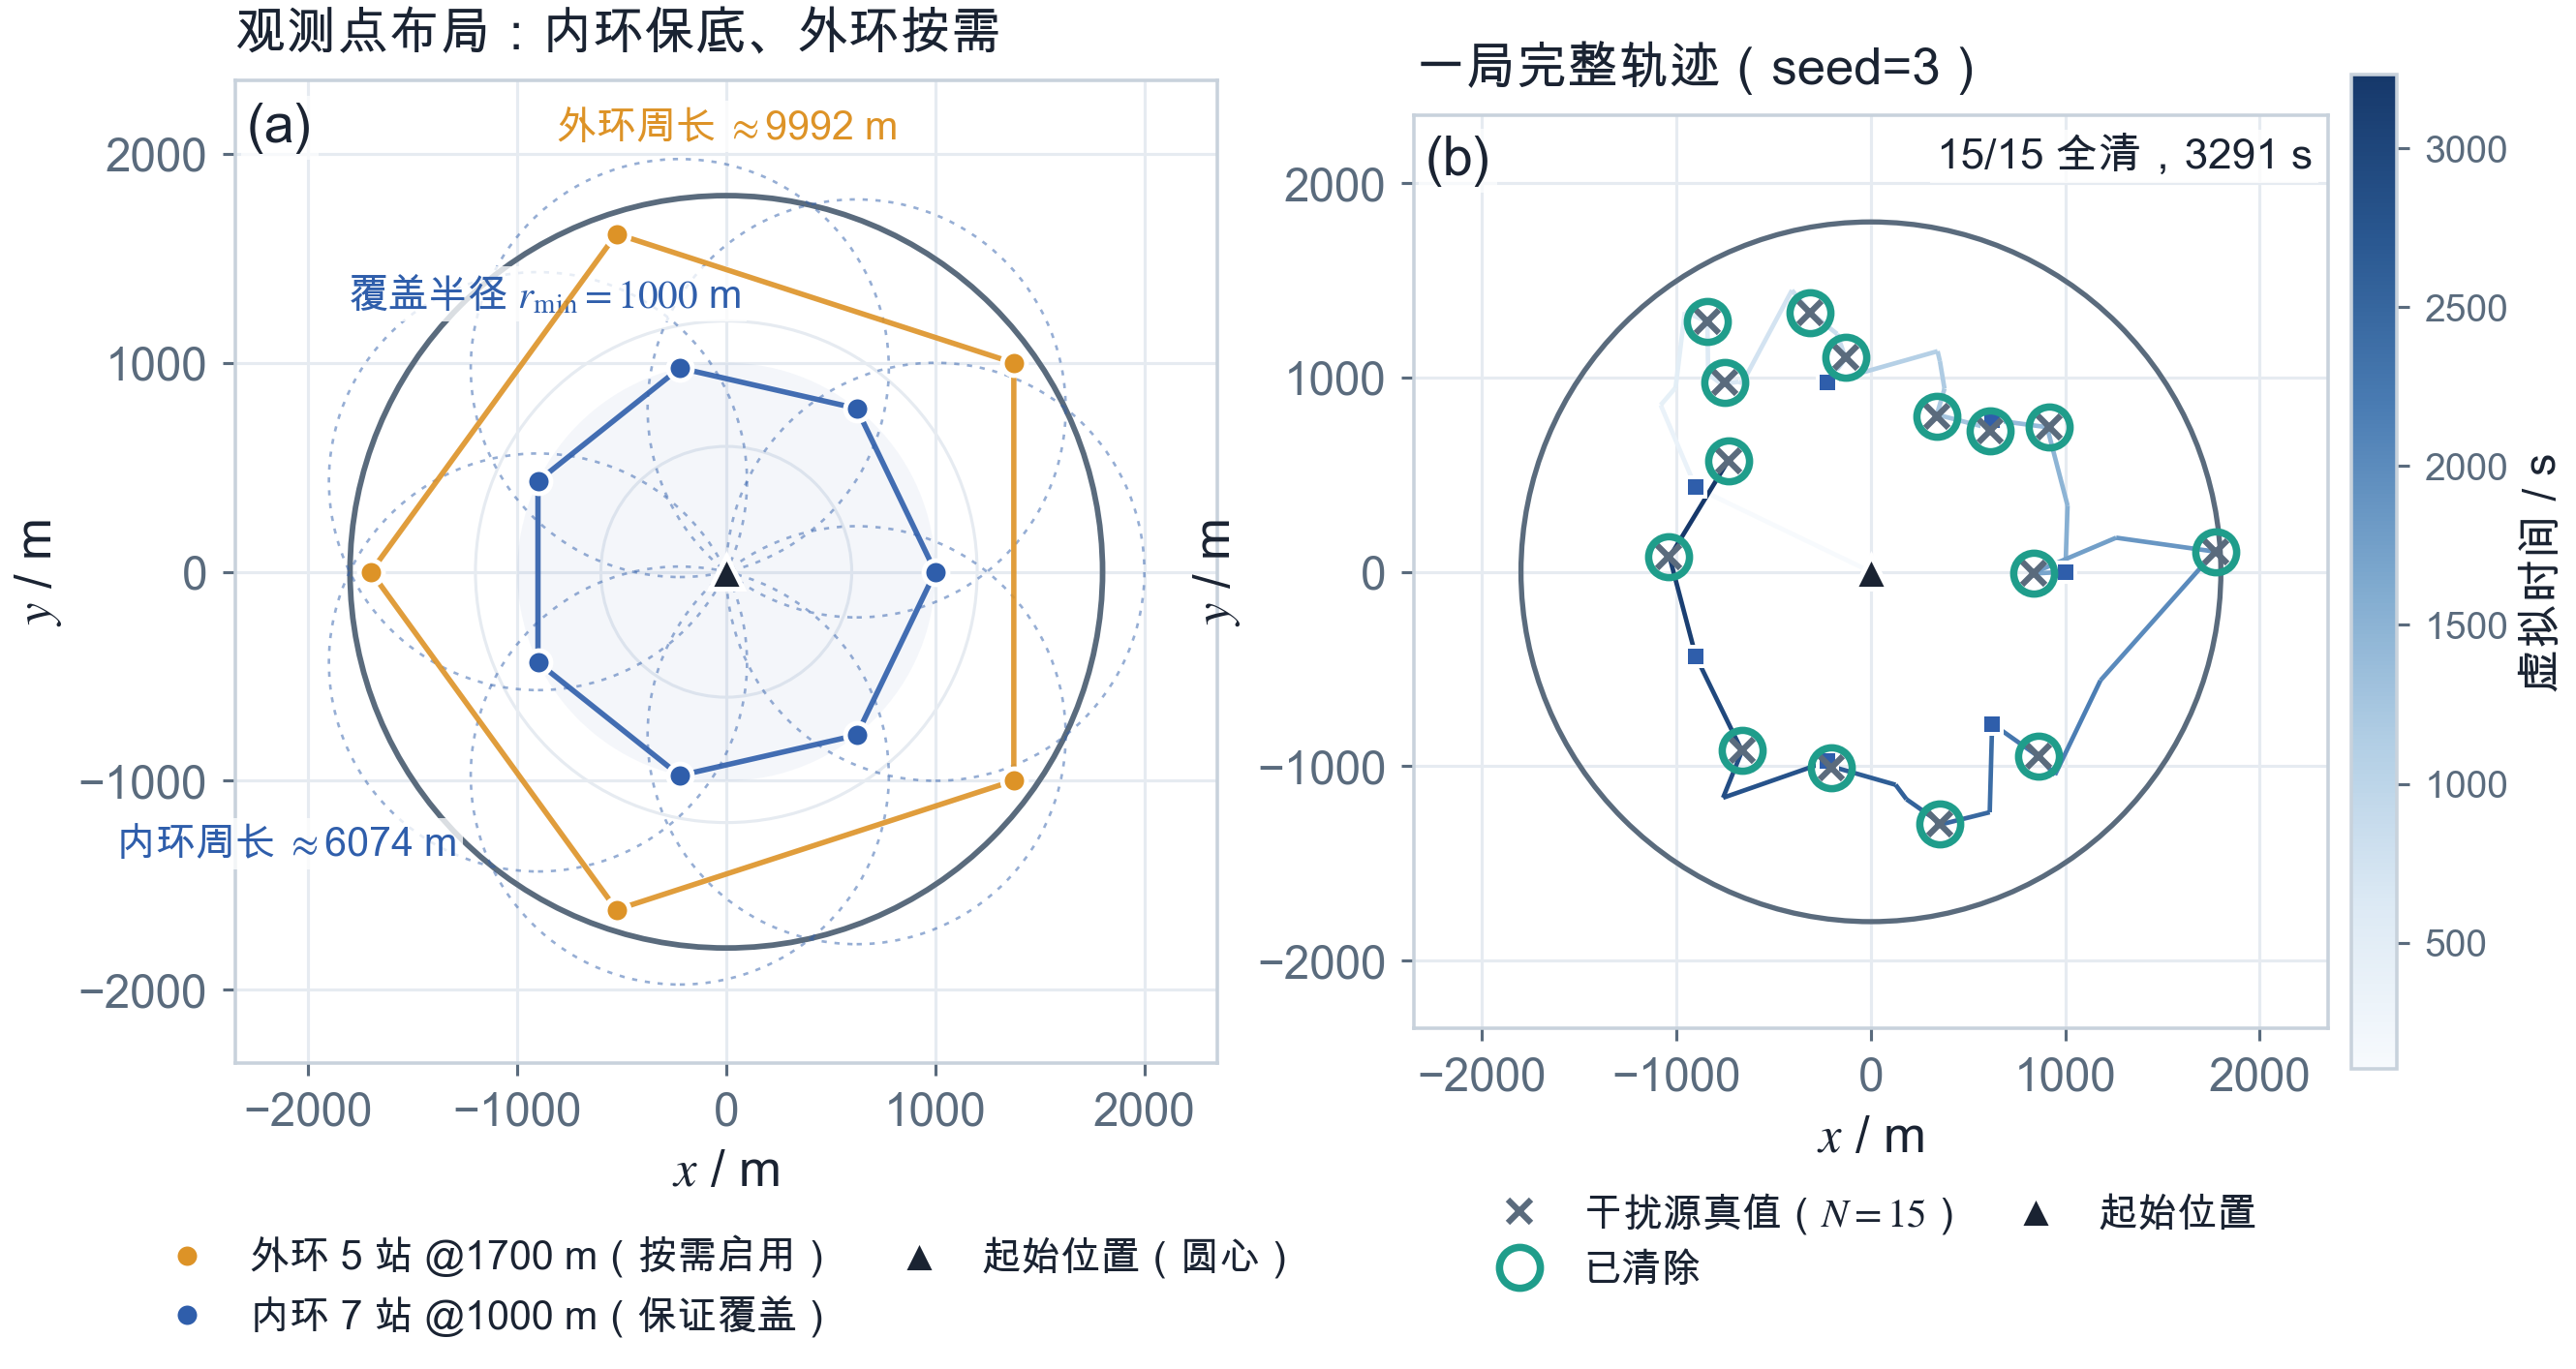
\includegraphics[width=0.95\textwidth]{B_fig4_q3_layout_path.png}
\caption{技术路线与观测点布局（左：内环保证覆盖、外环捕捉朝内定向源；右：一局完整轨迹）}
\label{fig:route}
\end{figure}

\begin{enumerate}
  \item \textbf{步骤一（问题一）}：把"一次检测"翻译成有序半平面约束，得到凸可行域 $\Reg$；把"不确定度"定义为 $\diam(\Reg)$，并给出其算法；回答"直径圆是否覆盖"给出 Thales 判据与 Jung 上界。
  \item \textbf{步骤二（问题二）}：以 $\diam$ 为损失，在"接收保证"约束下最大化第二次观测的信息增益，解出最优观测点。
  \item \textbf{步骤三（问题三）}：把 $\diam$ 作为"是否转入清剿"的阈值，设计"观测点布局 $+$ 滚动重规划调度"，用自建等价模拟器做大规模蒙卡演练。
  \item \textbf{步骤四（问题四）}：识别定向源带来的非凸性与几何盲区，给出零成本的定向源判据与自适应双环策略。
\end{enumerate}

\section{模型假设与符号说明}

\subsection{模型假设}

\begin{itemize}
  \item[A1] 示向度误差 $\varepsilon(P)\in[-1^\circ,1^\circ]$ 是位置的确定性函数（同点重复检测完全一致），本文所有推断只用该硬界，不假设其分布形式。
  \item[A2] 干扰源位置 $G_k\in\Arena$ 在测试期内静止，且\textbf{已知其位于目标区域内}（题面给出区域范围），故可行域一律与 $\Arena$ 求交。
  \item[A3] 有效接收半径 $r_k\in[1000,1500]$ m，逐源独立未知；凡出现 \texttt{direction} 即知 $|PG_k|\le1500$（因为 $r_k\le1500$）。
  \item[A4] 机器狗位置可精确控制并瞬时到达指定坐标（移动耗时按 $d/5$ 计），路径为空间折线。
  \item[A5] 各频道完全解耦：对某频道的检测不受其他频道干扰源影响。
  \item[A6] 定向源辐射只在主方向两侧各 $90^\circ$ 内有效；\texttt{/clear} 的光学精确定位与方向无关。
  \item[A7] 源个数 $N$ 在 $[10,16]$ 上等可能（用于论证"下限 $10$"与"上限 $16$"两类终止条件）。
\end{itemize}

\subsection{符号说明}

\begin{table}[H]
\centering
\caption{主要符号}
\label{tab:sym}
\small
\begin{tabular}{cl@{\qquad}cl}
\toprule
符号 & 含义 & 符号 & 含义 \\
\midrule
$\Arena$ & 目标区域（半径 $1800$ m 圆盘） & $D(\Reg)$ & 凸区域 $\Reg$ 的直径 \\
$G_k$ & 第 $k$ 个干扰源的位置 & $\Reg$ & 定位可行域（凸多边形） \\
$r_k$ & 第 $k$ 个源的有效接收半径 & $R_{\MEC}$ & $\Reg$ 的最小包围圆半径 \\
$\varphi_k$ & 定向源主方向 & $a,\ m$ & 观测环半径与站数 \\
$P_i,\ \theta_i$ & 第 $i$ 个观测点及其测得示向度 & $\rho,\ \alpha$ & 第二观测点的距离与偏角 \\
$\varepsilon$ & 示向度误差（$|\varepsilon|\le1^\circ$） & $\jj(S_2)$ & 第二点选择的目标函数 \\
$T$ & 定位清除总时间（优化目标） & $P_{\rm fail}$ & 第二点收不到信号的概率 \\
$L$ & 总路程 & $d$ & 源到第一观测点的距离 \\
\bottomrule
\end{tabular}
\end{table}

\medskip
\noindent\textbf{符号复用说明}：$\rho,\alpha$ 在问题二指第二观测点的极坐标（$\rho=|S_1S_2|$、$\alpha$ 为其相对示向度的偏角）；在问题四的阴影几何（第~\ref{sec:q4} 节）中 $\rho=|OG|$ 改指\emph{源的位置半径}，$\alpha$ 为源的辐射主方向角、$\beta$ 为观测站方位角，$\delta$ 为主方向与径向的夹角。请按节区分。

\medskip
\noindent 总时间可写为四项之和：
\begin{equation}
T=\underbrace{5M}_{\text{检测}}+\underbrace{N_{\rm sw}}_{\text{换频道}}+\underbrace{3F+5S}_{\text{清除}}+\underbrace{L/5}_{\text{移动}},
\label{eq:T}
\end{equation}
其中 $M$ 为检测次数、$N_{\rm sw}$ 为换频道次数、$F/S$ 为失败/成功清除次数。\textbf{移动项 $L/5$ 通常是主导项}（实测占比 $79\%$），因此策略设计的核心是把路程压到接近 TSP 下界。

\section{问题一：定位区域及其直径的算法}

\subsection{一次检测的信息：有序半平面约束}

设机器狗在 $P=(x_P,y_P)$ 处对某频道检测，测得示向度 $\theta$（以 $x$ 轴正向为 $0^\circ$，逆时针为正）。由洞察 1、2：

\begin{itemize}
  \item 若返回 \texttt{direction}：真实源 $G$ 满足
  \begin{equation}
  G\in\Wedge(P,\theta)\cap\overline{B(P,R_{\max})},\qquad
  \Wedge(P,\theta)=\Bigl\{Q:\bigl|\angle(Q-P)-\theta\bigr|\le 1^\circ\Bigr\},
  \end{equation}
  其中 $R_{\max}=1500$ m。"落在 $\pm1^\circ$ 楔形内"等价于 $G$ 同时位于\textbf{两条边界射线的同侧}：
  \begin{equation}
  (G-P)^{\!\top} n_\pm\ \ge\ 0,\qquad
  n_\pm=\pm\Bigl(-\sin(\theta\mp1^\circ),\ \cos(\theta\mp1^\circ)\Bigr),
  \label{eq:wedge}
  \end{equation}
  其中法向符号由"楔内测试点"唯一确定（取 $P+300(\cos\theta,\sin\theta)$ 代入取正）。\textbf{这一点很容易出错}：不能凭边界点判符号，否则会把楔形方向翻转。
  \item 若返回 \texttt{near}：$|G-P|\le5$ m，得到 $\overline{B(P,5)}$ 这一小圆盘约束（且可立即原地清剿）。
  \item 若返回 \texttt{no\_signal}：对全向源得 $|G-P|>r_k\ge1000$，是凹约束，本文在问题一至三中\textbf{保守地丢弃}该信息（不用会略微放大区域，但保证不产生漏解）；在问题四中该信息被重新启用，见第~\ref{sec:q4} 节。
\end{itemize}

于是 $n$ 次检测后的定位可行域为凸多边形的交集
\begin{equation}
\boxed{\ \Reg=\Arena\ \cap\ \bigcap_{i=1}^{n}\Bigl(\Wedge(P_i,\theta_i)\cap\overline{B(P_i,R_{\max})}\Bigr)}
\label{eq:region}
\end{equation}
（\texttt{near} 时对应的 $\overline{B(P_i,5)}$ 取代 $\Wedge\cap\overline{B}$）。

\subsection{直径算法}

$\Reg$ 是凸多边形，设其顶点（已按逆时针排序）为 $V_1,\dots,V_n$（$n$ 通常为 $3\!\sim\!6$）。

\noindent\textbf{算法 1（凸多边形直径）}
\begin{enumerate}
  \item \textbf{裁剪}：从覆盖全域的大圆内接 $K$ 边形（本文 $K=144$）出发，对式~\eqref{eq:region} 中每个约束按 Sutherland--Hodgman 做半平面裁剪，圆盘用内接正多边形近似（$K=72$ 边形，误差 $<0.1\%$）。复杂度 $O(nK)$。
  \item \textbf{顶点枚举}：$\diam=\max_{1\le i<j\le n}\|V_i-V_j\|$，$O(n^2)$。由于 $n$ 很小，本文直接用枚举；若 $n$ 很大可用旋转卡壳降到 $O(n)$。
  \item \textbf{退化保护}：若某次裁剪后顶点数 $<3$，判定为\textbf{约束不相容}（例如方位矛盾），说明检测数据异常或源已被清除，该频道进入待复核队列。
\end{enumerate}

\noindent\textbf{算法 2（最小包围圆）} 本文用 Welzl 增量法（等价的三点/两点枚举实现）：直径圆的圆心取两个最远点中点，若不能覆盖全部顶点，则最优圆由三个顶点外接确定。该量用于回答问题一的"圆是否覆盖"。

\subsection{"以定位区域直径为直径的圆"能否覆盖该区域}

设 $AB$ 为 $\Reg$ 的一对直径端点（$\|A-B\|=D$），记 $\mathcal D$ 为以 $AB$ 为直径的圆。

\begin{quote}
\textbf{命题 1（Thales 判据）} 设 $\Reg$ 为凸集，$AB$ 为其直径。则
\begin{equation}
\Reg\subseteq\mathcal D
\quad\Longleftrightarrow\quad
\forall V\in\operatorname{ext}(\Reg):\ \angle AVB\ \ge\ 90^\circ .
\label{eq:thales}
\end{equation}
\end{quote}

\noindent\textbf{证明} 由 Thales 定理，$\mathcal D=\{Q:\angle AQB\ge90^\circ\}$，且 $\mathcal D$ 是凸集。若所有极点满足 $\angle AVB\ge90^\circ$，则它们都在 $\mathcal D$ 中；$\Reg=\conv(\operatorname{ext}\Reg)$ 且 $\mathcal D$ 凸，故 $\Reg\subseteq\mathcal D$。反之若某极点 $V\notin\mathcal D$ 即 $\angle AVB<90^\circ$，则 $V\in\Reg$ 但 $V\notin\mathcal D$，覆盖不成立。$\square$

命题 1 给出一个 $O(n)$ 的\textbf{可判定判据}，同时说明问题一的答案是\textbf{"不必然覆盖"}：只要存在一个顶点使 $\angle AVB<90^\circ$ 即反例。

\medskip
\noindent\textbf{最坏情况有多坏？} 设 $R_{\MEC}$ 为 $\Reg$ 的最小包围圆半径。由 \textbf{Jung 定理}，对平面凸集
\begin{equation}
R_{\MEC}\ \le\ \frac{D}{\sqrt3}\ =\ 0.5774\,D
\qquad\Longrightarrow\qquad
\frac{R_{\MEC}}{D/2}\ \le\ \frac{2}{\sqrt3}=1.1547 .
\label{eq:jung}
\end{equation}
即\textbf{最坏情况下直径圆要比"够用"的圆小 $15.47\%$}。这是一个\textbf{普适上界}，与观测点个数无关。

\subsection{数值验证}

\noindent\textbf{（1）算例}。取 $S_1=(0,0)$、$S_2=(1200,300)$，真源 $G=(900,800)$，两次方位由 $G$ 精确给出（示向度 $41.63^\circ$、$120.96^\circ$）。计算结果：

\begin{center}
\small
\begin{tabular}{cccccc}
\toprule
直径 $D$ & 最小包围圆 $R_{\MEC}$ & $R_{\MEC}/(D/2)$ & 顶点数 & 最小张角 $\angle AVB$ & 判据 \\
\midrule
$50.88$ m & $25.44$ m & $1.0000$ & $4$ & $100.67^\circ$ & \textbf{成立} \\
\bottomrule
\end{tabular}
\end{center}

即此算例中 $\mathcal D$ 恰好覆盖 $\Reg$（$R_{\MEC}=D/2$），最小张角 $100.67^\circ\ge90^\circ$ 与命题 1 自洽。图~\ref{fig:q1} 左给出可行域、直径、直径圆与最小包围圆；右为逐顶点张角检验。

\begin{figure}[H]
\centering
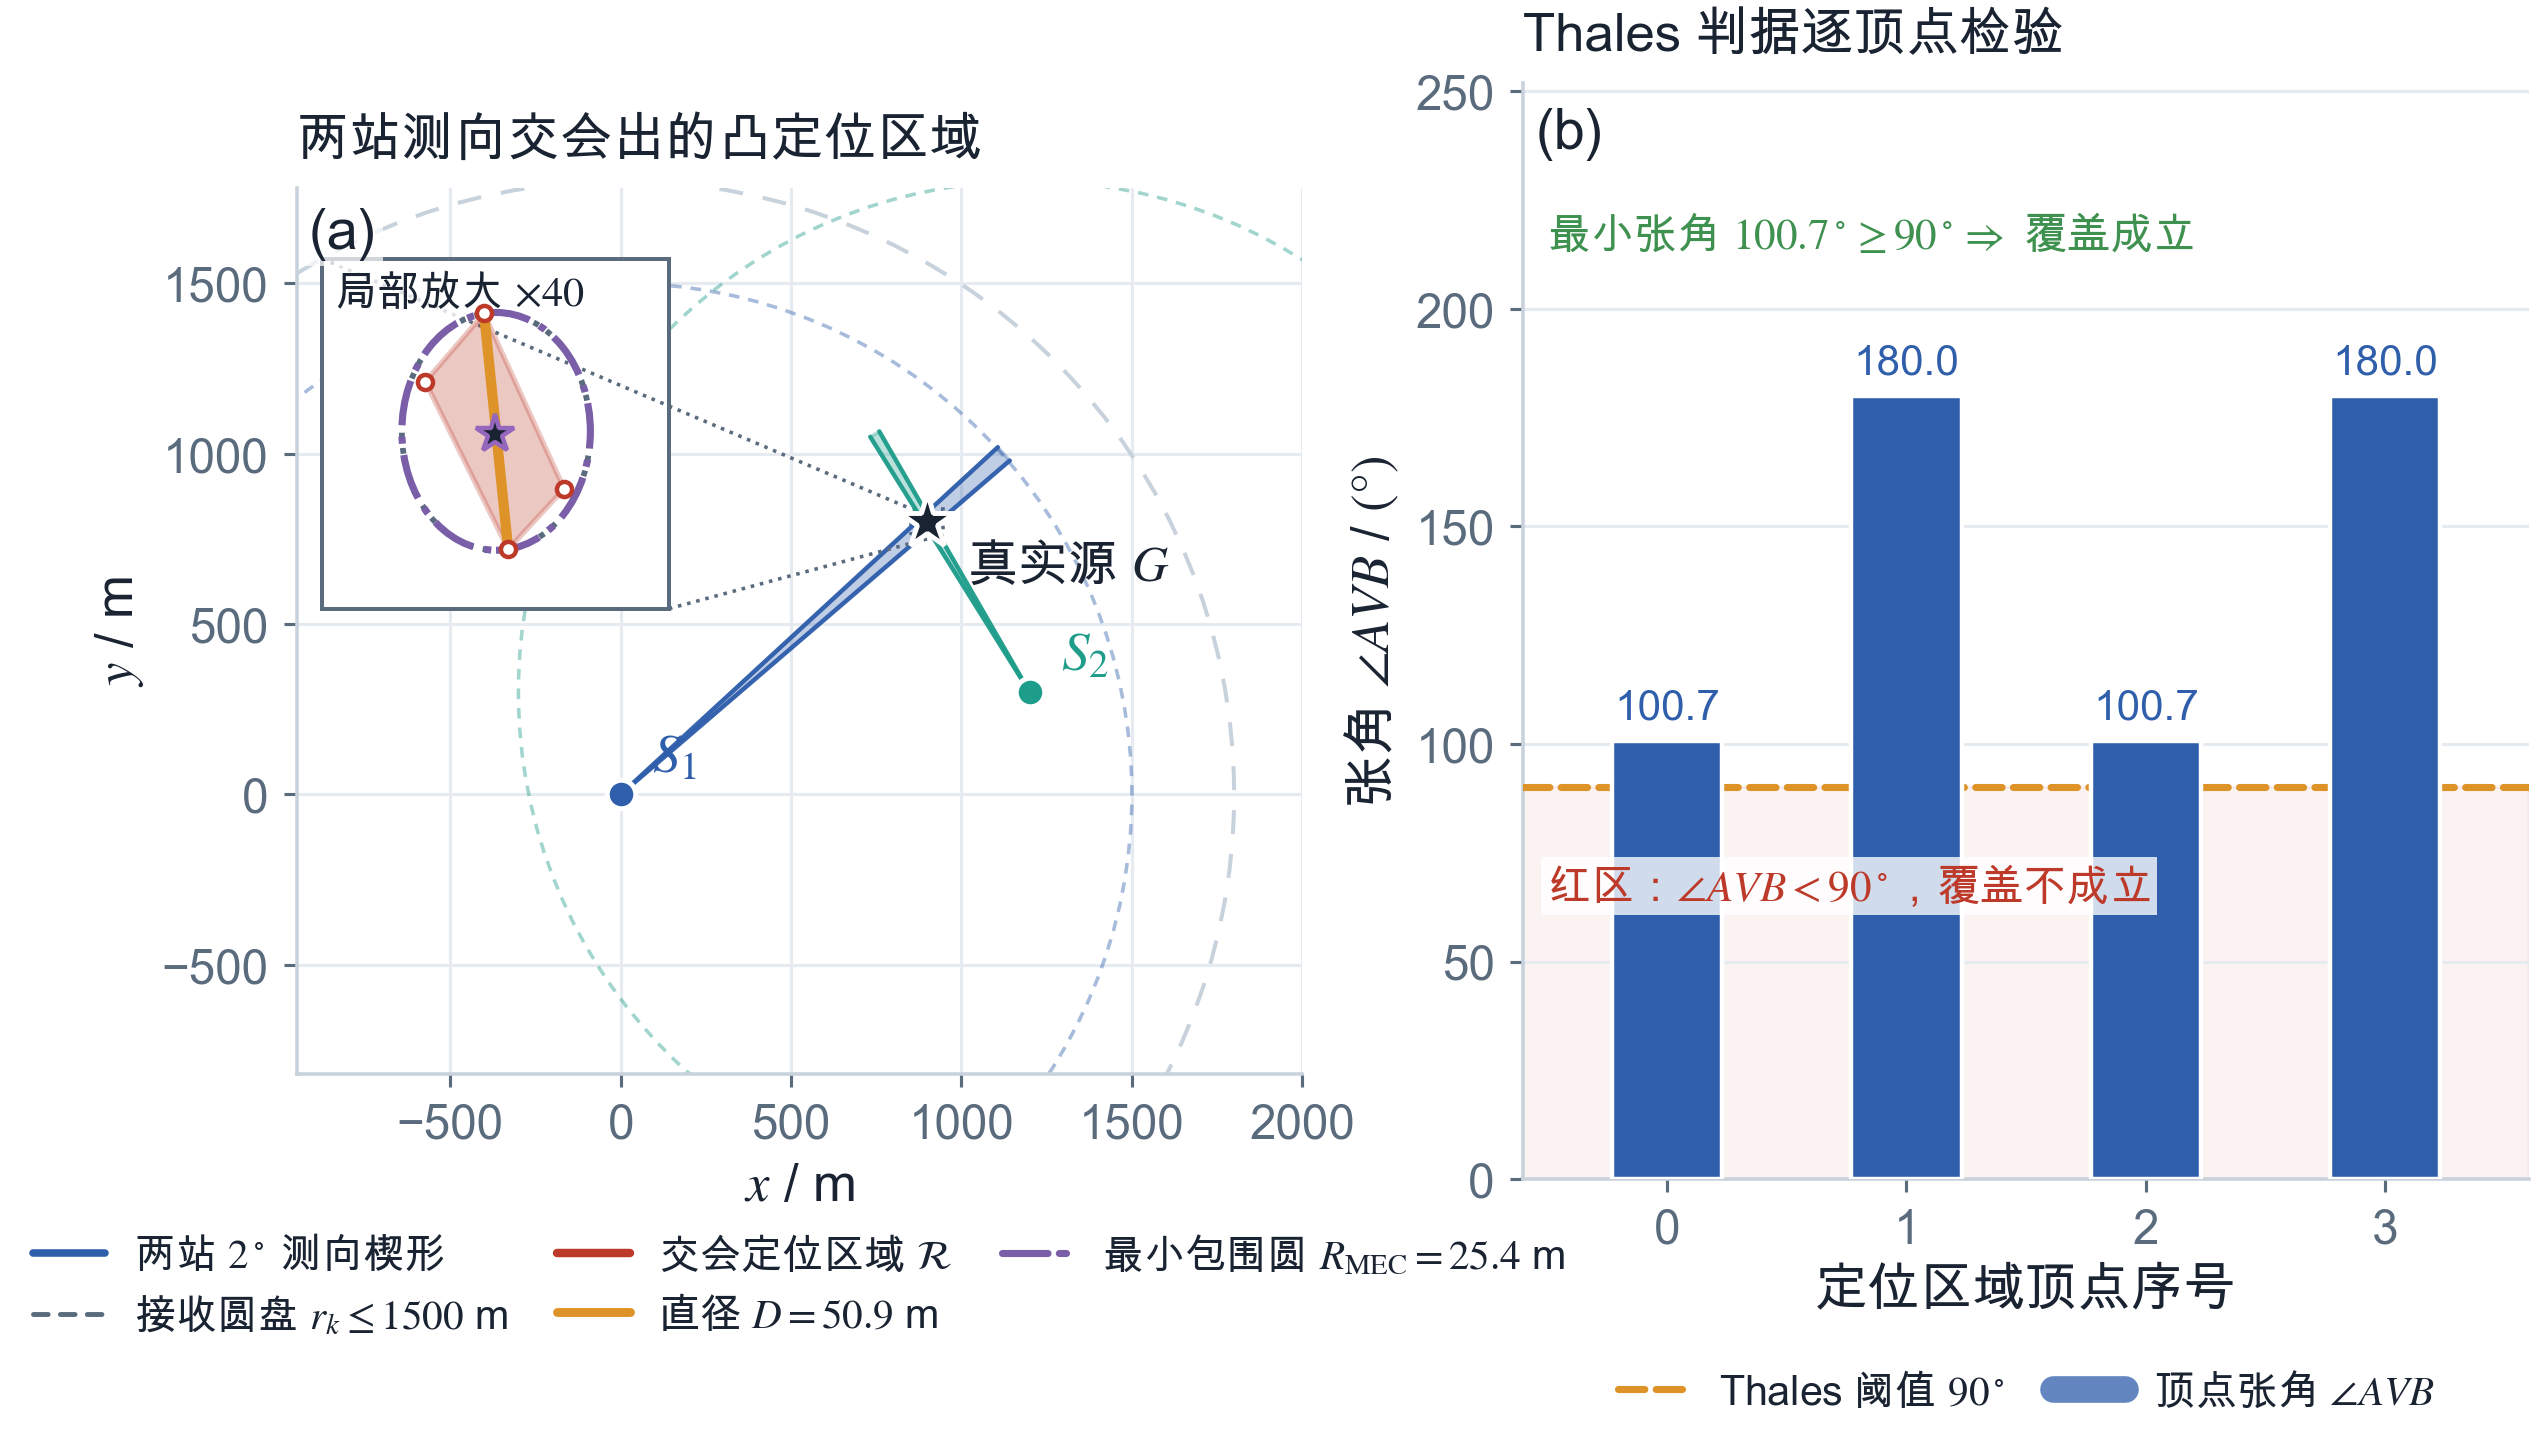
\includegraphics[width=\textwidth]{B_fig1_q1_region.png}
\caption{问题一算例：(a) 两次检测的 2$^\circ$ 楔形交会出的凸可行域、其直径 $D$、以 $D$ 为直径的圆与最小包围圆；(b) 按命题 1 逐顶点检验 $\angle AVB\ge90^\circ$}
\label{fig:q1}
\end{figure}

\noindent\textbf{（2）最坏情况搜索}。对观测点个数 $m=2,3,4,5$ 各做 $4\times10^4$ 次随机构型抽样（首站置于原点，其余站方位 $U[0,2\pi)$、半径 $U[300,2800]$；源在半径 $1650$ m 内均匀；要求所有站与源距离不超过 $1500$ m 且不小于 $30$ m，即"全部站都测得到"），统计 $R_{\MEC}/(D/2)$：

\begin{table}[H]
\centering
\caption{随机构型下 $R_{\MEC}/(D/2)$ 的实测分布（各 $4\times10^4$ 次抽样）}
\label{tab:jung}
\small
\begin{tabular}{ccccc}
\toprule
观测点个数 $m$ & 有效样本 & 实测最大值 & 超出 $D/2$ 的最大幅度 & $99.9\%$ 分位 \\
\midrule
$2$ & $9\,598$  & $1.0148$ & $+1.48\%$ & $1.0030$ \\
$3$ & $3\,934$  & $1.0941$ & $+9.41\%$ & $1.0255$ \\
$4$ & $1\,572$  & $1.0674$ & $+6.74\%$ & $1.0283$ \\
$5$ & $636$    & $1.0511$ & $+5.11\%$ & $1.0390$ \\
\midrule
\multicolumn{2}{c}{Jung 上界（与 $m$ 无关）} & $1.1547$ & $+15.47\%$ & --- \\
\bottomrule
\end{tabular}
\end{table}

最严重构型出现在 $m=3$：检测点 $(0,0)$、$(147.3,895.8)$、$(-572.7,-327.8)$，真源 $(-1149.6,959.5)$，此时 $D=56.0$ m、$R_{\MEC}=30.6$ m、比值 $1.0941$。

\begin{figure}[H]
\centering
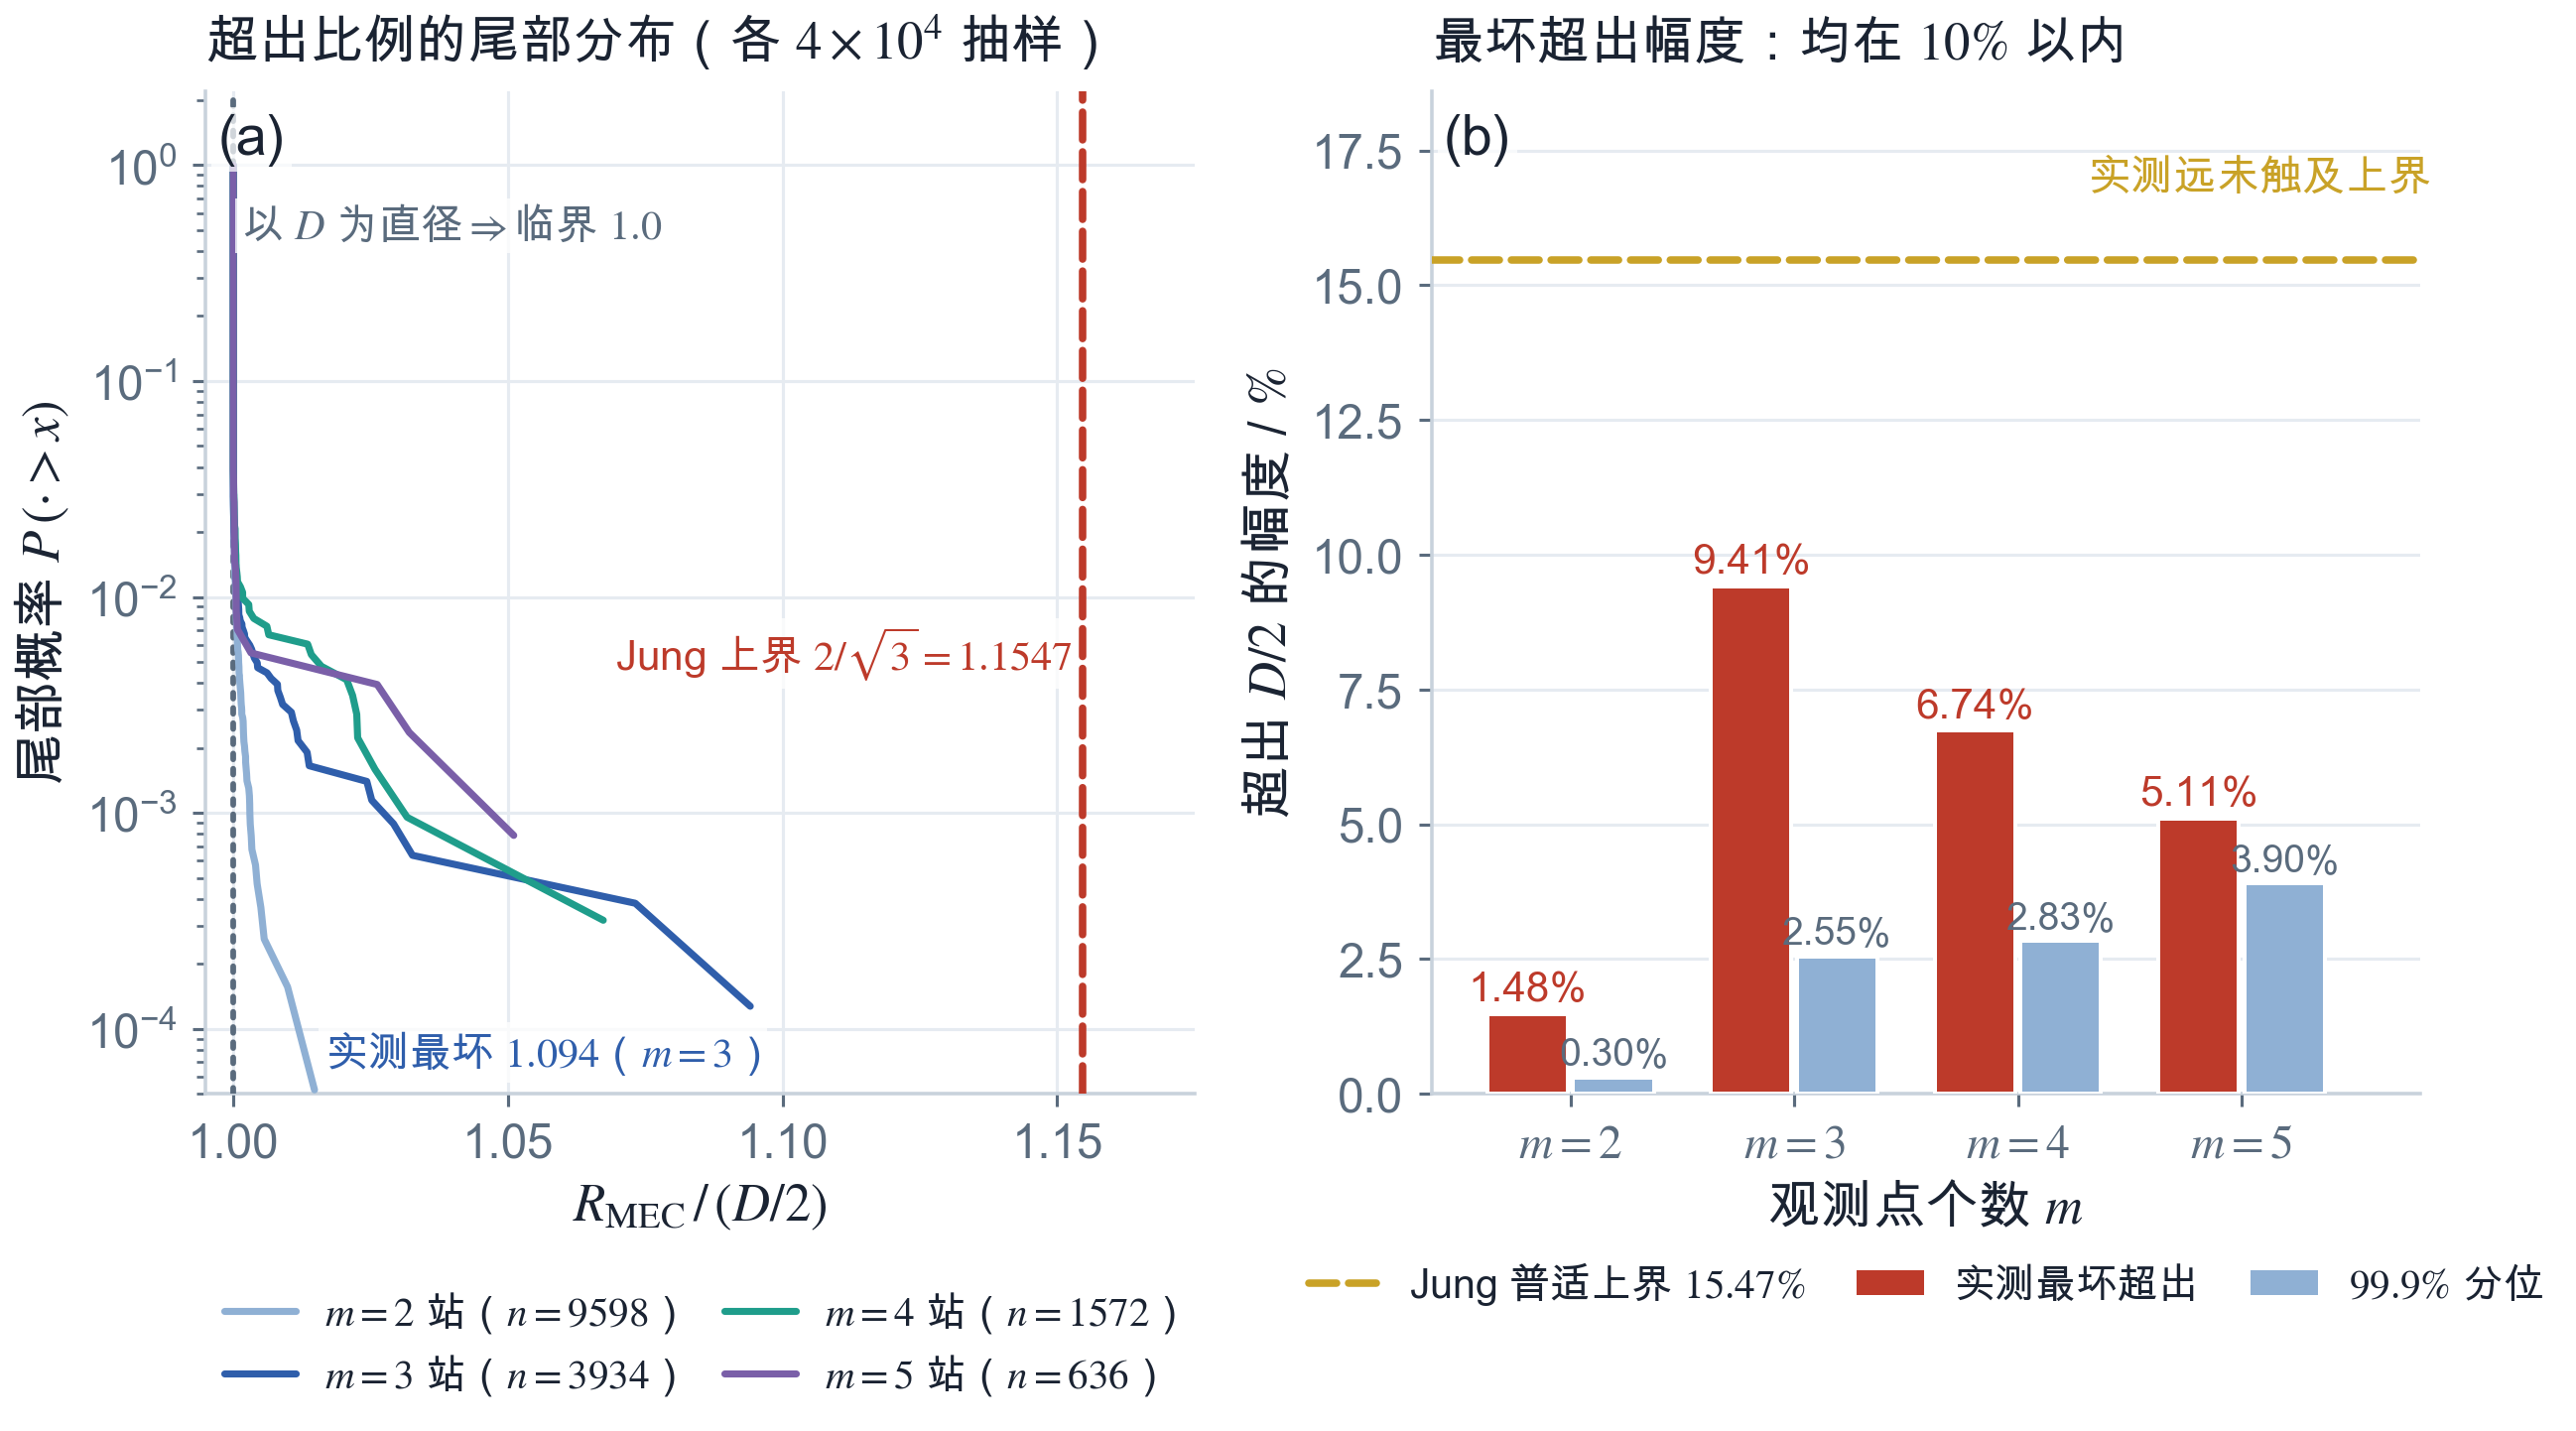
\includegraphics[width=\textwidth]{B_fig2_q1_jung.png}
\caption{问题一最坏情况：(a) $R_{\MEC}/(D/2)$ 的分布；(b) 实测最坏幅度随站数变化，均远低于 Jung 上界}
\label{fig:jung}
\end{figure}

\noindent\textbf{结论}：
\begin{enumerate}
  \item 以定位区域直径为直径的圆\textbf{不必然}覆盖该区域；严格判据是命题 1 的 Thales 条件。
  \item 但\textbf{实际中几乎总成立}：$2$ 站交会（题目图 2 的情形）最坏也只超出 $1.48\%$，$3\!\sim\!5$ 站最坏 $5\%\!\sim\!9\%$，全部远小于 Jung 上界 $15.47\%$。因此\textbf{在小概率极端几何下，用直径作"覆盖半径"会低估，工程上应改用 $R_{\MEC}$（或以 $D/\sqrt3$ 作保守设计值）}。
  \item 站数 $m$ 越大，$R_{\MEC}/(D/2)$ 的分布反而略宽（因为可选构型更多），但有效样本数急剧下降——这意味着"多站同时可见"本身是稀缺事件，与问题四中"定向源常只有 1 站可见"的现象一致。
\end{enumerate}

\section{问题二：第二检测点的最优选择策略}

\subsection{把"定位效果好"翻译成可优化的目标函数}

由问题一，\textbf{定位精度就是可行域的直径 $\diam(\Reg)$}。选择第二检测点 $S_2$ 时，我们面对两个互相冲突的效应：

\begin{itemize}
  \item \textbf{效应 A（条件数）}：$S_2$ 离 $S_1$ 越远、与示向度夹角越大，两条方位线交会角越大，$\diam$ 越小；
  \item \textbf{效应 B（接收保证）}：源距离 $d$ 未知，$S_2$ 一旦偏离示向度方向，就可能\textbf{收不到信号}——此时第二次检测\textbf{完全没有信息}，区域直径停留在仅一次测量的水平。
\end{itemize}

于是目标函数取"第二次测量后的期望直径"，并对"收不到"施以惩罚（惩罚值取仅一次方位时的不确定度上界 $R_{\max}=1500$ m）：

\begin{equation}
\boxed{\ \jj(S_2)=\underbrace{P_{\rm fail}(S_2)}_{\text{第二次无信号}}\cdot R_{\max}
\ +\ \underbrace{\E\bigl[\diam(\Reg_2)\ \big|\ \text{成功}\bigr]}_{\text{成功时的期望直径}}\ }
\label{eq:J}
\end{equation}

\subsection{源距离的先验分布}

$S_1$ 能测到该源 $\Longrightarrow$ $d\le r_k$ 且 $d\ge5$。$r_k\sim U[1000,1500]$，故

\begin{equation}
P(r_k\ge d)=\begin{cases}1,& d\le1000,\\[2pt]
\dfrac{1500-d}{500},& 1000<d<1500,\\[2pt] 0,& d\ge1500,\end{cases}
\qquad
\pi(d)\ \propto\ \underbrace{d}_{\text{面积元}}\cdot P(r_k\ge d),\quad d\in[5,1500].
\label{eq:prior}
\end{equation}

\textbf{注意 $\pi(d)\propto d$ 这一点至关重要}：由于源在圆盘内均匀、半径大的圆环面积大，$d$ 的先验偏向大值（数值上 $\E[d]\approx855$ m）。这解释了为什么"保守地假设源就在附近"会导致完全错误的结论。

\subsection{关键约束：保证接收}

设 $S_1$ 至源的方向为 $\theta_1=0$（旋转不变性），$|S_1S_2|=\rho$，$S_2$ 相对示向度的偏角为 $\alpha$。要\textbf{保证}（对最不利的 $r_k=1000$ m 也成立）$S_2$ 能收到该源，需

\begin{equation}
\begin{aligned}
|S_2G|^2&=\rho^2-2\rho d\cos\alpha+d^2\ \le\ r_{\min}^2=1000^2\\
&\Longleftarrow\quad
\rho\in\Bigl[d\cos\alpha-\sqrt{r_{\min}^2-d^2\sin^2\alpha},\ d\cos\alpha+\sqrt{r_{\min}^2-d^2\sin^2\alpha}\Bigr].
\end{aligned}
\end{equation}

该区间存在当且仅当 $d|\sin\alpha|\le r_{\min}$，即

\begin{equation}
\boxed{\ |\alpha|\ \le\ \alpha_{\max}(d)\ :=\ \arcsin\!\bigl(r_{\min}/d\bigr)\ }
\label{eq:alphamax}
\end{equation}

\textbf{对偶形式（图~\ref{fig:q2}(a) 所绘）}：若反过来固定第二点距离 $\rho$、只让源距 $d$ 变化，则同一二次式的判别式给出的条件是把 $d$ 与 $\rho$ 互换，即存在能（在最不利的 $r_k=r_{\min}$ 下）被 $S_2$ 接收的源距当且仅当 $\rho|\sin\alpha|\le r_{\min}$：

\begin{equation}
\boxed{\ |\alpha|\ \le\ \arcsin\!\bigl(r_{\min}/\rho\bigr)\ }
\label{eq:dualbound}
\end{equation}

这在 $(\rho,\alpha)$ 平面上给出"保证接收"的可行边界——因为 $|S_2G|^2$ 对 $d$ 取极小值为 $\rho^2\sin^2\alpha$，故 $\rho\sin\alpha>r_{\min}$ 的方案无论真实源落在哪个半径上、$S_2$ 都收不到信号。这也解释了图~\ref{fig:q2}(a) 的机理：$\rho$ 越大，允许的偏角越小，可行域是一条向原点张开的楔形。

数值上：$d\le r_{\min}=1000$ m 时 $\alpha_{\max}\ge90^\circ$（此时任意偏角都有某个 $\rho$ 能保证收到）；$d$ 越大约束越紧，$d=1200$ m 时 $\alpha_{\max}=56.4^\circ$，$d=1300$ m 时 $50.3^\circ$，\textbf{当 $d\to1500$ m 时收敛到 $\arcsin(1000/1500)=41.8^\circ$}。\textbf{要害在于}：\textbf{纯侧移（$\alpha$ 接近 $90^\circ$）在几何上不可能收到远端源，其 $P_{\rm fail}$ 必然很大}，而由式~\eqref{eq:prior}，源恰有相当概率落在 $1300\!\sim\!1500$ m 的远端环带。

\subsection{数值求解与最优解}

对 $\rho\in[100,2800]$ m、$\alpha\in[0^\circ,180^\circ]$ 做 $100\times121$ 网格搜索，每次用两射线求交得到四边形的直径（射线求交必须\textbf{同时校验两个参数为非负}，否则会把反向延长线的虚交点算进来），结果：

\begin{equation}
\boxed{\ \alpha^*=31.5^\circ,\qquad \rho^*=1054\ \text{m},\qquad \jj^*=50.3\ \text{m}\ }
\end{equation}

$\jj\le1.05\jj^*$ 的候选带为 $|S_1S_2|\in[970,1150]$ m、$|\alpha|\in[25^\circ,40^\circ]$（左右镜像等价）。

\begin{figure}[H]
\centering
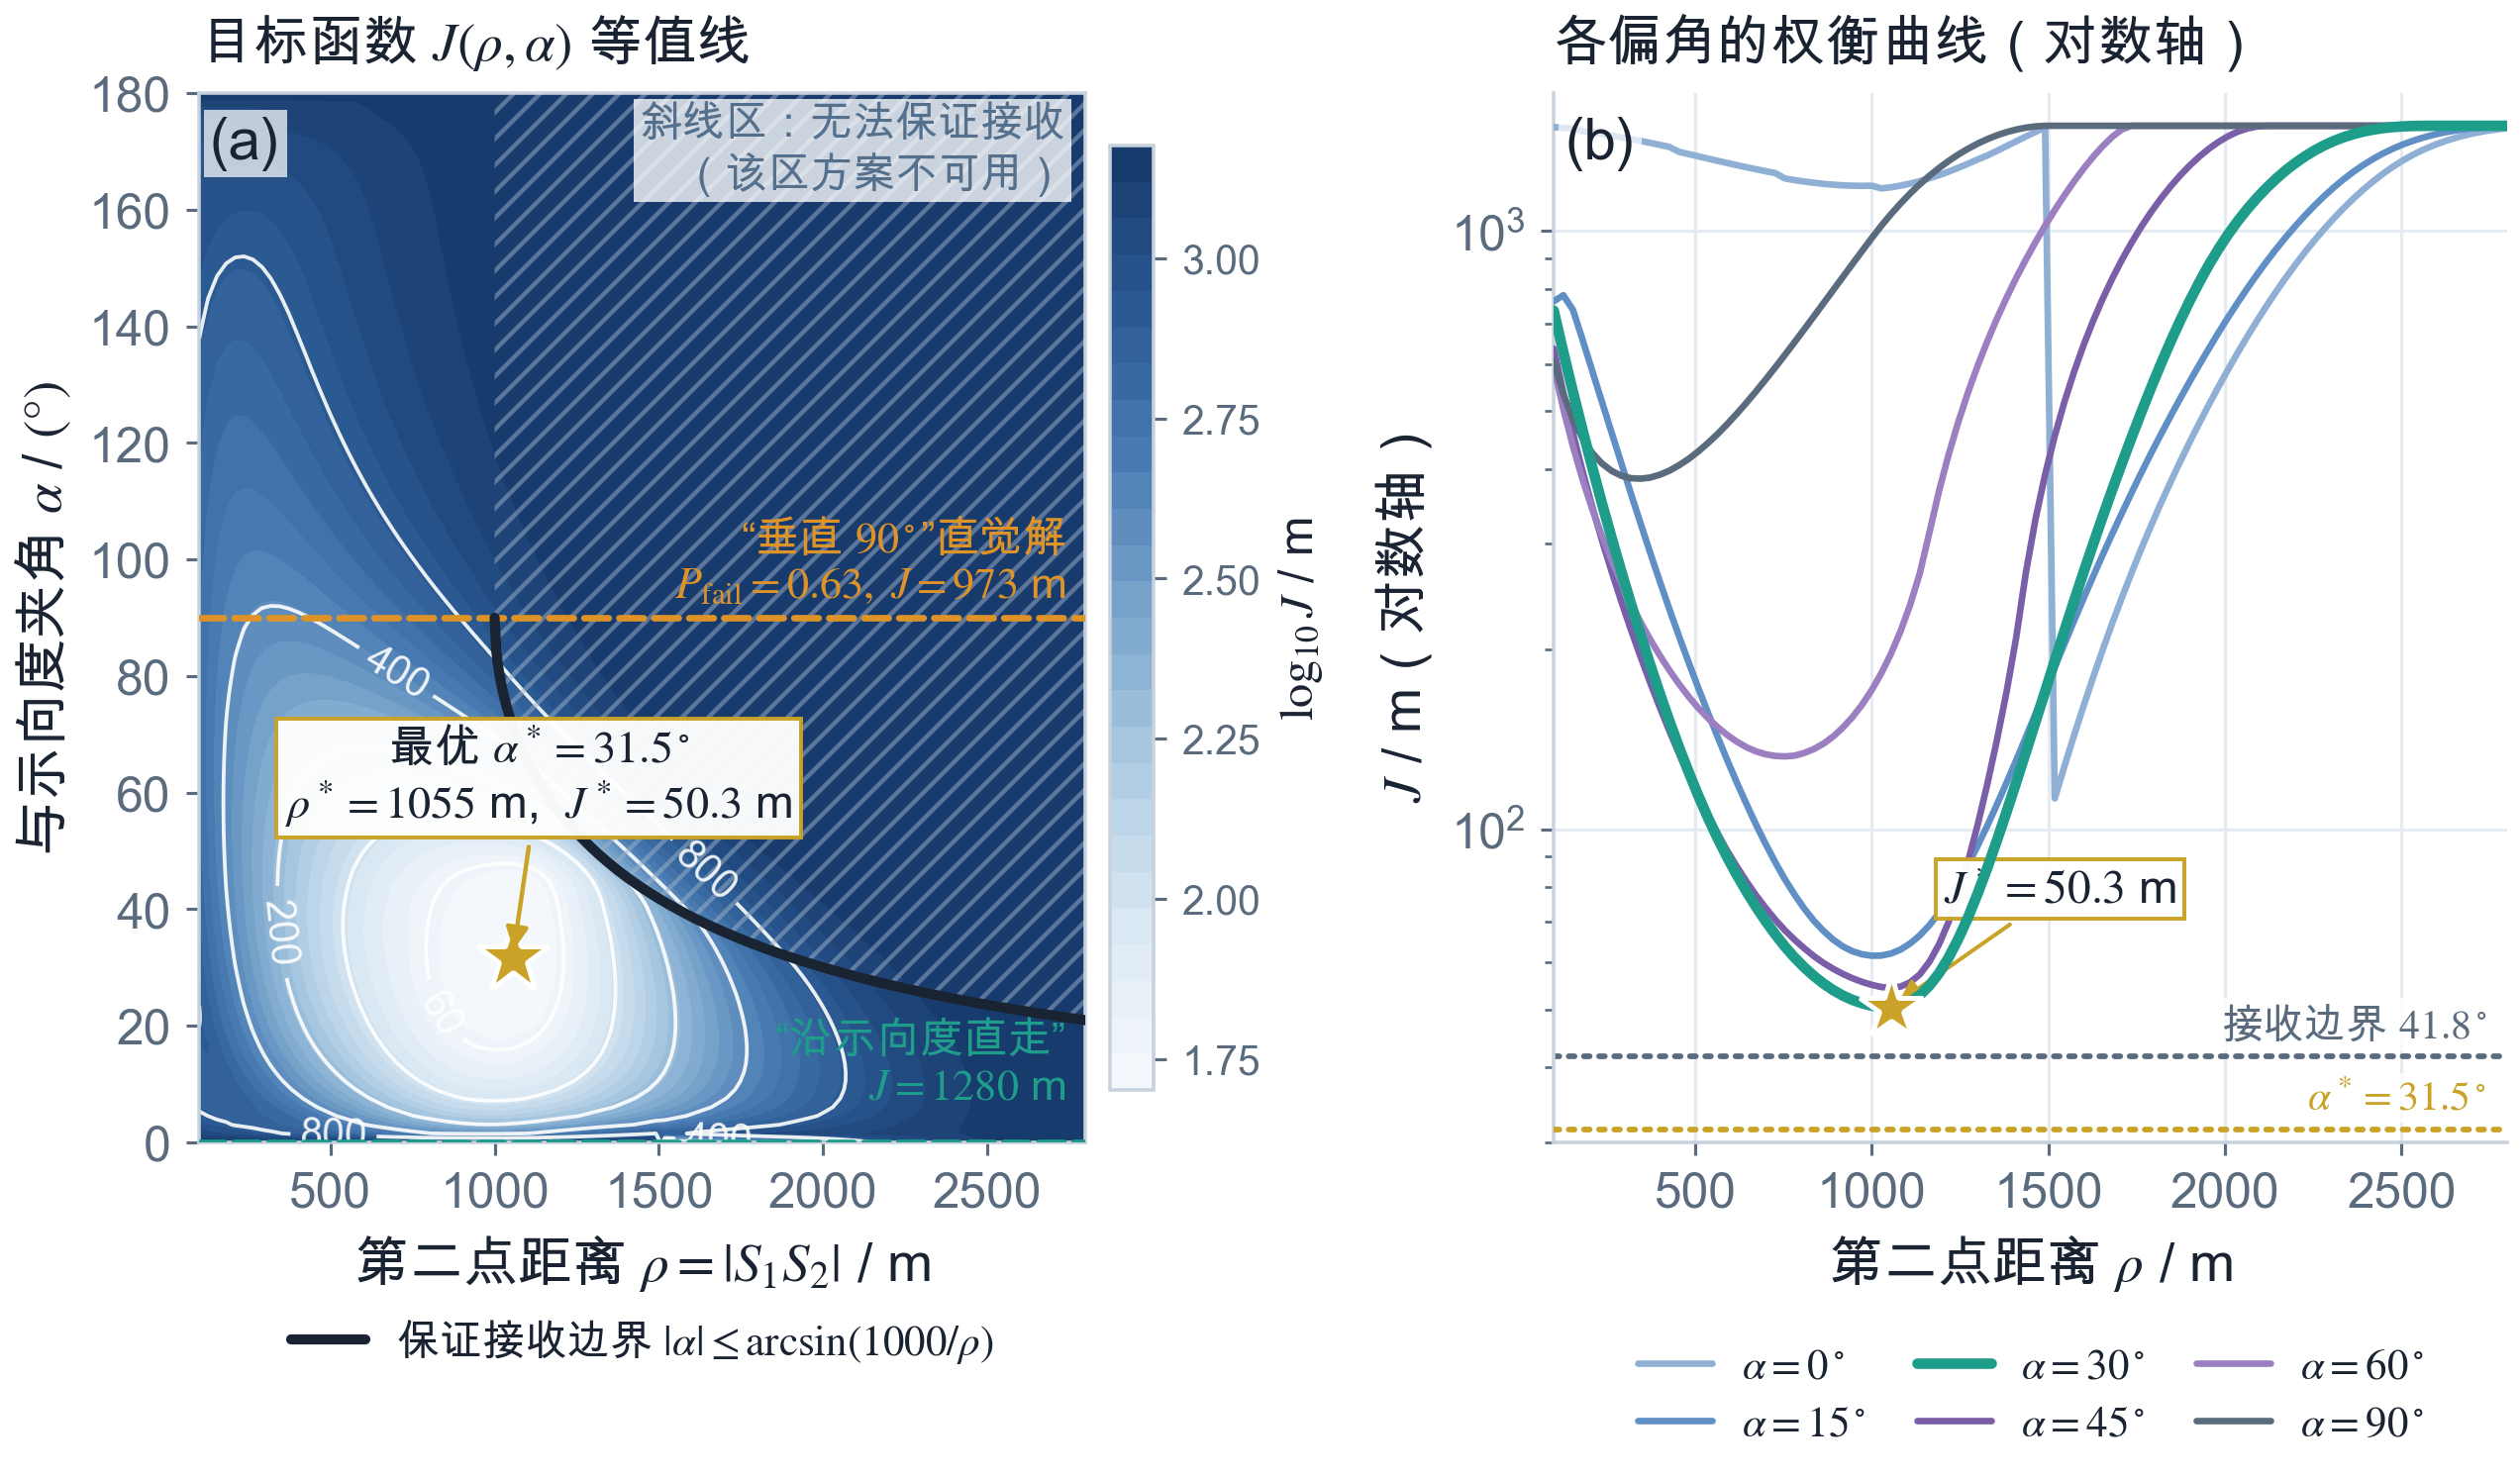
\includegraphics[width=\textwidth]{B_fig3_q2_design.png}
\caption{问题二：(a) 目标函数 $J(\rho,\alpha)$ 等值线，叠加保证接收的对偶边界 $|\alpha|\le\arcsin(1000/\rho)$ 与两个直觉解；(b) 各偏角下的权衡曲线（对数轴），$\alpha^*=31.5^\circ$ 附近有明确谷底}
\label{fig:q2}
\end{figure}

\subsection{两个必须澄清的反直觉结论}

\noindent\textbf{（1）"垂直 $90^\circ$"是错的。} 直觉上基线越宽越好，于是取 $\alpha=90^\circ$。但在 $d$ 的先验下：

\begin{center}
\small
\begin{tabular}{lccc}
\toprule
方案 & $P_{\rm fail}$ & 成功时平均直径 & $\jj$ \\
\midrule
垂直 $90^\circ$、$\rho=1000$ m & $0.633$ & --- & $973.3$ m \\
垂直 $90^\circ$、$\rho=1500$ m & $1.000$ & --- & $1500.0$ m \\
沿示向度直走 $\rho=1250$ m & $0.006$ & $1268$ m & $1280.2$ m \\
偏 $45^\circ$、$\rho=800$ m & $0.001$ & $62.7$ m & $63.9$ m \\
\textbf{最优：偏 $31.5^\circ$、$\rho=1054$ m} & $\mathbf{0.000}$ & $\mathbf{50.3}$ m & $\mathbf{50.3}$ m \\
偏 $20^\circ$、$\rho=1200$ m & $0.004$ & $64.4$ m & $64.6$ m \\
\bottomrule
\end{tabular}
\end{center}

$\alpha=90^\circ$ 时 $\rho=1000$ m 有 $63.3\%$ 的概率收不到信号（$\rho=1500$ m 时必失败），$J$ 高达 $973$ m，\textbf{是最优解的 $19$ 倍}。根因就是式~\eqref{eq:alphamax}。

\noindent\textbf{（2）"沿示向度方向直走"也是错的。} 此时两次观测点与源\textbf{近乎共线}，两条方位线几乎重合，交会角趋近 $0$，区域\emph{不收缩}：虽然几乎总能收到信号（$P_{\rm fail}=0.6\%$），但成功时直径仍有 $1268$ m，$\jj=1280$ m，\textbf{是最优解的 $25$ 倍}。

\noindent\textbf{（3）最优解的物理解释}：$\alpha^*\approx30^\circ$ 恰是"用尽量大的交会角换取尽量高的接收概率"的折中点；$\rho^*\approx1054$ m 则约为 $r_{\min}=1000$ m 的量级——再远则超出有效接收半径的风险上升，再近则交会基线太短、$\diam\propto d\,\delta\theta/\sin(\angle)$ 的误差放大因子变大。

\subsection{可直接执行的选择策略}

\begin{quote}
\textbf{策略 Q2}（设第一观测点 $S_1$、测得示向度 $\theta_1$）：
\begin{enumerate}
  \item 沿 $\theta_1$ 取 $S_1$ 前方 $R_{\text{aux}}=1000$ m 处的参考点 $C=S_1+1000(\cos\theta_1,\sin\theta_1)$（即承诺区域质心的近似）；
  \item 取第二观测点
  \begin{equation}
  S_2=C+\rho^*\Bigl(\cos(\theta_1\pm\alpha^*),\ \sin(\theta_1\pm\alpha^*)\Bigr),\quad
  \rho^*=1050\ \text{m},\ \alpha^*=30^\circ,
  \end{equation}
  符号取使 $S_2$ 仍落在目标区域（或合法坐标域）内的一侧；两侧均合法时任取一侧；
  \item 若 $S_2$ 处返回 \texttt{no\_signal}，\textbf{不要}沿示向度方向试探，而是\textbf{镜像到另一侧} $-\alpha^*$ 补测一次（因 $\varphi$ 先验均匀，阴影侧等概率，镜像的成功率约为 $50\%\to$ 显著改善）；
  \item 若两侧均无信号，退化为"径向前进"策略：把 $S_2$ 沿 $\theta_1$ 推进到 $1300\!\sim\!1500$ m 处再测（牺牲条件数换接收率），并同时在\textbf{反方向}（$\theta_1+180^\circ$）测一次以排除方位翻转。
\end{enumerate}
\end{quote}

该策略在问题三中被直接实现为"主动定位点"子算法（第~\ref{sec:q3} 节），并在问题四中被进一步修正为"中等深度双向探测"（第~\ref{sec:q4} 节）。

\section{问题三：全向干扰源的最短时间搜索—清除策略}
\label{sec:q3}

\subsection{先算清"下界"，再谈"优化"}

由式~\eqref{eq:T}，时间由四部分构成。我们先把"任何策略都无法避免"的部分算出来，才能判断一个方案是否接近最优。

\noindent\textbf{（i）覆盖下界。} 设在半径 $a$ 的圆环上布 $m$ 个等角观测点。由于有效接收半径下界 $r_{\min}=1000$ m，\textbf{要保证任意位置的源都能被至少一个观测点收到}，需满足
\begin{equation}
\underbrace{a\ \le\ 1000}_{\text{圆心处}},\qquad
\underbrace{a^2-2Ra\cos\tfrac{\pi}{m}+R^2\ \le\ r_{\min}^2}_{R=1800,\ \text{相邻两站连线中点处}} .
\label{eq:cover}
\end{equation}
第二式给出 $a\in[a_-(m),a_+(m)]$，其中 $a_\pm=R\cos\frac{\pi}{m}\pm\sqrt{R^2\cos^2\frac{\pi}{m}-(R^2-r_{\min}^2)}$。求解：

\begin{table}[H]
\centering
\caption{保证覆盖所需的最小站数（$r_{\min}=1000$ m，$R=1800$ m）。环周长与巡回路程由 \texttt{q3\_bounds.py} 复算}
\label{tab:cover}
\small
\setlength{\tabcolsep}{3.4pt}
\resizebox{\linewidth}{!}{%
\begin{tabular}{lcccccc}
\toprule
$m$ & $5$ & $6$ & $7$ & $8$ & $9$ & $12$ \\
\midrule
可行 $a$ 区间 & $\varnothing$ & $[1123,1995]$ & $[997.2,\,2246.3]$ & $[938.1,\,2387.9]$ & $[903.4,\,2479.5]$ & $[853.8,\,2623.5]$ \\
与 $a\leq1000$ 求交 & $\varnothing$ & $\varnothing$ & $[997.2,\,1000]$ & $[938.1,\,1000]$ & $[903.4,\,1000]$ & $[853.8,\,1000]$ \\
环周长（$a{=}1000$ m）/ m & --- & --- & $\bm{6074}$ & $6123$ & $6156$ & $6212$ \\
自圆心入环巡回路程 / m & --- & --- & $\bm{7074}$ & $7123$ & $7156$ & $7212$ \\
\bottomrule
\end{tabular}%
}
\end{table}

\textbf{结论：$m=6$ 时两式矛盾（要求 $a\ge1123$ 且 $a\le1000$），保证覆盖的等角圆环最少需要 $7$ 个观测点。} 这是一个必须写清的\textbf{负结论}：它说明"少布几个点、多扫几遍"在几何上不可行，站数的下界是 $7$ 而不是 $4$（按面积算 $\lceil R^2/r_{\min}^2\rceil=4$ 只是必要不充分条件）。注意 $m=7$ 时 $a$ 的可行区间\emph{极窄}（$997.3\!\sim\!1000$ m），这决定了实际布站应取 $a\approx1000$ m（贴近该窄区间的上端）；若把 $a$ 压到 $925$ m 以下，虽在 $r_k>1000$ m 的多数情形下仍能覆盖，但$r_k$ 取下界的最不利情形会失去保证。

\noindent\textbf{（ii）检测下界。} 一次全频段扫描 $20$ 个频道需
\begin{equation}
t_{\rm sweep}=20\times5+19\times1=119\ \text{s}.
\end{equation}

\noindent\textbf{（iii）路程下界（oracle）。} 若机器狗事先知道全部源位置，则最优路程是"起点$\,+\,$全部源"的旅行商问题；但本问必须走访覆盖环才能发现源，故\textbf{可比的标尺}是"起点$\,+\,$源$\,+\,$覆盖环 $7$ 站"的合并路线。用最近邻 $+$ 2-opt（多起点重启，$n\le17$ 时通常即最优）求解，$50$ 组随机构型（$N$ 取 $10/13/16$）平均（\texttt{q3\_bounds.py}）：

\begin{center}
\small
\setlength{\tabcolsep}{5pt}
\begin{tabular}{lccc@{\qquad}c}
\toprule
& $N=10$ & $N=13$ & $N=16$ & 三档平均 \\
\midrule
理想下界：起点$\,+\,$源 & $8216$ m & $9608$ m & $10\,531$ m & $9452$ m $=1890$ s \\
\textbf{有效下界：起点$\,+\,$源$\,+\,$覆盖环 $7$ 站} & $10\,253$ m & $11\,541$ m & $12\,813$ m & $\bm{11\,536}$ m $\bm{=2307}$ s \\
\bottomrule
\end{tabular}
\end{center}

因此\textbf{理想情况下的时间下界约 $1890$ s}；而对"必须走访全部覆盖环"的策略，\textbf{真正的参照是 $2307$ s}。后文即以此标尺衡量。

\noindent\textbf{（iv）为什么不能"先全覆盖再清剿"。} 一个自然的想法是"先把 $7$ 个站扫完拿到全部源位置，再规划清剿路线"。我们用 \texttt{order\_ablation.py} 做单因子对照（全向、$50$ 局，只切换 \texttt{two\_pass} 开关）：两趟式路程 $15\,567$ m、总时间 $3929$ s、检测 $124.3$ 次；滚动重规划 $14\,765$ m、$3661$ s、$106.2$ 次，即\textbf{路程省 $5.1\%$、时间省 $6.8\%$、检测次数省 $14.6\%$}。收益有两个来源：清剿目标与扫描站在空间上交错，两趟式被迫往返；而边扫边清还能\textbf{避免对同一频道的重复扫描}（先扫时只拿到方位，回头清剿仍需补测）。因此正确做法是把扫描与清剿放进同一条路径，边扫边清（下文算法）。

\subsection{\texorpdfstring{算法总览：三层任务 $+$ 滚动重规划}{算法总览：三层任务 + 滚动重规划}}

我们把每个频道的状态记为 $(\Reg_k,\ n_k^{\rm dir},\ n_k^{\rm loc},\ \text{cleared}_k)$，其中 $\Reg_k$ 为式~\eqref{eq:region} 的可行域、$n^{\rm dir}$ 为有效方位数、$n^{\rm loc}$ 为主动定位次数。

\medskip
\noindent\textbf{算法 3（滚动重规划 Rolling Re-planning）}

每一步都做三件事：

\textbf{Step 1 —— 生成候选任务集}（三类）：
\begin{equation}
\mathcal T=\underbrace{\{S_i:\ \text{未扫的观测站}\}}_{\text{扫}}
\ \cup\ \underbrace{\{c_k:\ \diam(\Reg_k)\le D_{\rm ready}\}}_{\text{清剿}}
\ \cup\ \underbrace{\{L_k:\ \text{几何病态待补测}\}}_{\text{主动定位}} .
\end{equation}

\textbf{Step 2 —— 滚动 TSP 选点}：以当前位置为起点，对 $\mathcal T$ 的"代表点"（站取自身坐标，清剿取可行域质心，定位取式~\eqref{eq:loc} 的探测点）做最近邻 $+$ $2$-opt，\textbf{只执行巡回的第一站}，随后丢弃整个排序、按新信息重排。这一"视界为 1"的设计使算法能立刻响应"扫描某站后突然有多个频道变可清剿"的事件。

\textbf{Step 3 —— 执行该动作并更新}$\Reg$：清扫一个站 $\to$ 对未跳过频道逐个 \texttt{/measure}；若返回 \texttt{near} 则原地 \texttt{/clear}（零移动代价）。清剿一个频道 $\to$ 见 6.4。主动定位 $\to$ 见 6.4。

\medskip
\noindent\textbf{跳过规则（节省检测次数）}：在观测站 $S$ 上，若频道 $k$ 已有方位且 $\diam(\Reg_k)\le D_{\rm skip}=45$ m，说明其位置已足够精确，\textbf{不再检测}。这使得 $7$ 个站的总检测次数从 $140$ 次降到约 $110$ 次。

\noindent\textbf{终止规则}：$\text{n}_{\rm det}$（已获得方位数的频道数）达到题目上限 $16$ 时立即停止一切扫描；否则扫完 7 站后进入"补测"循环。

\subsection{子算法}

\noindent\textbf{（a）可行域更新。} 见式~\eqref{eq:wedge}--\eqref{eq:region}，用 Sutherland--Hodgman 裁剪，圆盘用 $72$ 边形近似，$O(nK)$ 且数值稳定。\texttt{near} 时把该频道的可行域直接收缩为半径 $5$ m 的小圆盘。

\noindent\textbf{（b）主动定位点（问题二结论的工程落地）。} 当某频道只有 $1$ 个方位时，$\Reg_k$ 是一条沿视线的窄楔形，$\diam\approx1300$ m，永远不会触发清剿。此时取第二个探测点
\begin{equation}
L_k=P_0+t\,u+\sigma\,\delta\,w,\qquad u=\frac{C-P_0}{\|C-P_0\|},\ w\perp u,\ \ t=0.35\!\sim\!0.6\,t_{\max},\ \delta=t/2,
\label{eq:loc}
\end{equation}
其中 $P_0$ 为最近一次观测点、$C$ 为 $\Reg_k$ 质心、$t_{\max}$ 为区域在视线方向的最大延伸、$\sigma=\pm1$ 为正反两侧。交会角 $\theta\approx\arctan(\delta/t)\approx27^\circ$，足以把 $\diam$ 从 $1300$ m 压到数十米。

\begin{quote}
\textbf{这里有一个致命陷阱}（问题一/二的几何知识直接救场）：若按"区域质心（即视线末端 $\sim$1000 m 深处）$+\,$侧移 $200$ m"取点，交会角只有 $\arctan(200/1000)\approx11^\circ$，\textbf{区域几乎不收缩，且对定向源会整片落入阴影}。因此必须取\textbf{中等深度}（$t\approx0.35\!\sim\!0.6\,t_{\max}$）而不是末端。第~\ref{sec:q4} 节将看到这一细节对问题四成败的决定性作用。
\end{quote}

\noindent\textbf{（c）清剿。} 当 $\diam(\Reg_k)\le D_{\rm ready}=100$ m 时，按 $24$ m 间距在 $\Reg_k$ 内生成网格候选点（$24<\sqrt2\cdot20$，保证网格点的 $20$ m 覆盖圆盘能盖住整片区域），按"离当前位置由近及远"依次 \texttt{/clear}；全部失败后改为"以质心为中心、半径 $18$ m 的 $12$ 点环"再扫一圈作为兜底。清剿失败时把阈值收紧（$D_{\rm ready}/(1+2f)$，$f$ 为失败次数），避免在错误区域反复消耗。

\subsection{自建等价模拟器与计时校验}

官方模拟器仅提供 Windows 64 位版本（\texttt{Jammers-simulator-win64.7z}），无法在当前环境运行。我们依据题面附录 1/2 与附件 1《模拟器使用说明》、附件 2《通信接口说明及编程指南》\textbf{用 Python 复刻了语义完全等价的模拟器}，包括：

\begin{itemize}
  \item 四条指令 \texttt{/enter}、\texttt{/measure}、\texttt{/clear}、\texttt{/exit} 与 HTTP 状态码、字段合法性校验（未声明字段 $\to$ \texttt{accepted=false}，缺字段 $\to$ HTTP $400$，\texttt{robot\_id}/\texttt{arena\_id} 校验）；
  \item \textbf{request\_id 幂等性}：同 id 同内容返回首次响应；同 id 改内容返回 $409$。客户端只在重试时复用原 id；
  \item \textbf{虚拟计时}：移动 $d/5$、换频道 $1$ s、检测 $5$ s、清除 $3/5$ s，且 \texttt{/clear} 不改变测向机当前频道（因此后续 \texttt{/measure} 可能\textbf{不}产生切换耗时）——这是最容易实现错的一条；
  \item 三种返回语义（\texttt{direction}$+$\texttt{svd\_deg} / \texttt{near} / \texttt{no\_signal}）、$20$ m 清除半径、\texttt{near} 阈值 $5$ m、定向源半平面覆盖。
\end{itemize}

\noindent\textbf{校验}：附件 1 表 2 的示例给出了逐条指令后的虚拟时刻 $105$、$111$、$194$、$199$ s（其中第 $5$ 步因前一步 \texttt{/clear} 未切换频道而不产生切换耗时）。自建模拟器\textbf{逐秒复现了这四个时刻}，说明计时规则实现正确。程序中策略与模拟器通过统一的 \texttt{transport} 接口解耦，把 \texttt{LocalTransport} 换成 \texttt{HttpTransport} 即可直接对官方模拟器运行。

\begin{figure}[H]
\centering
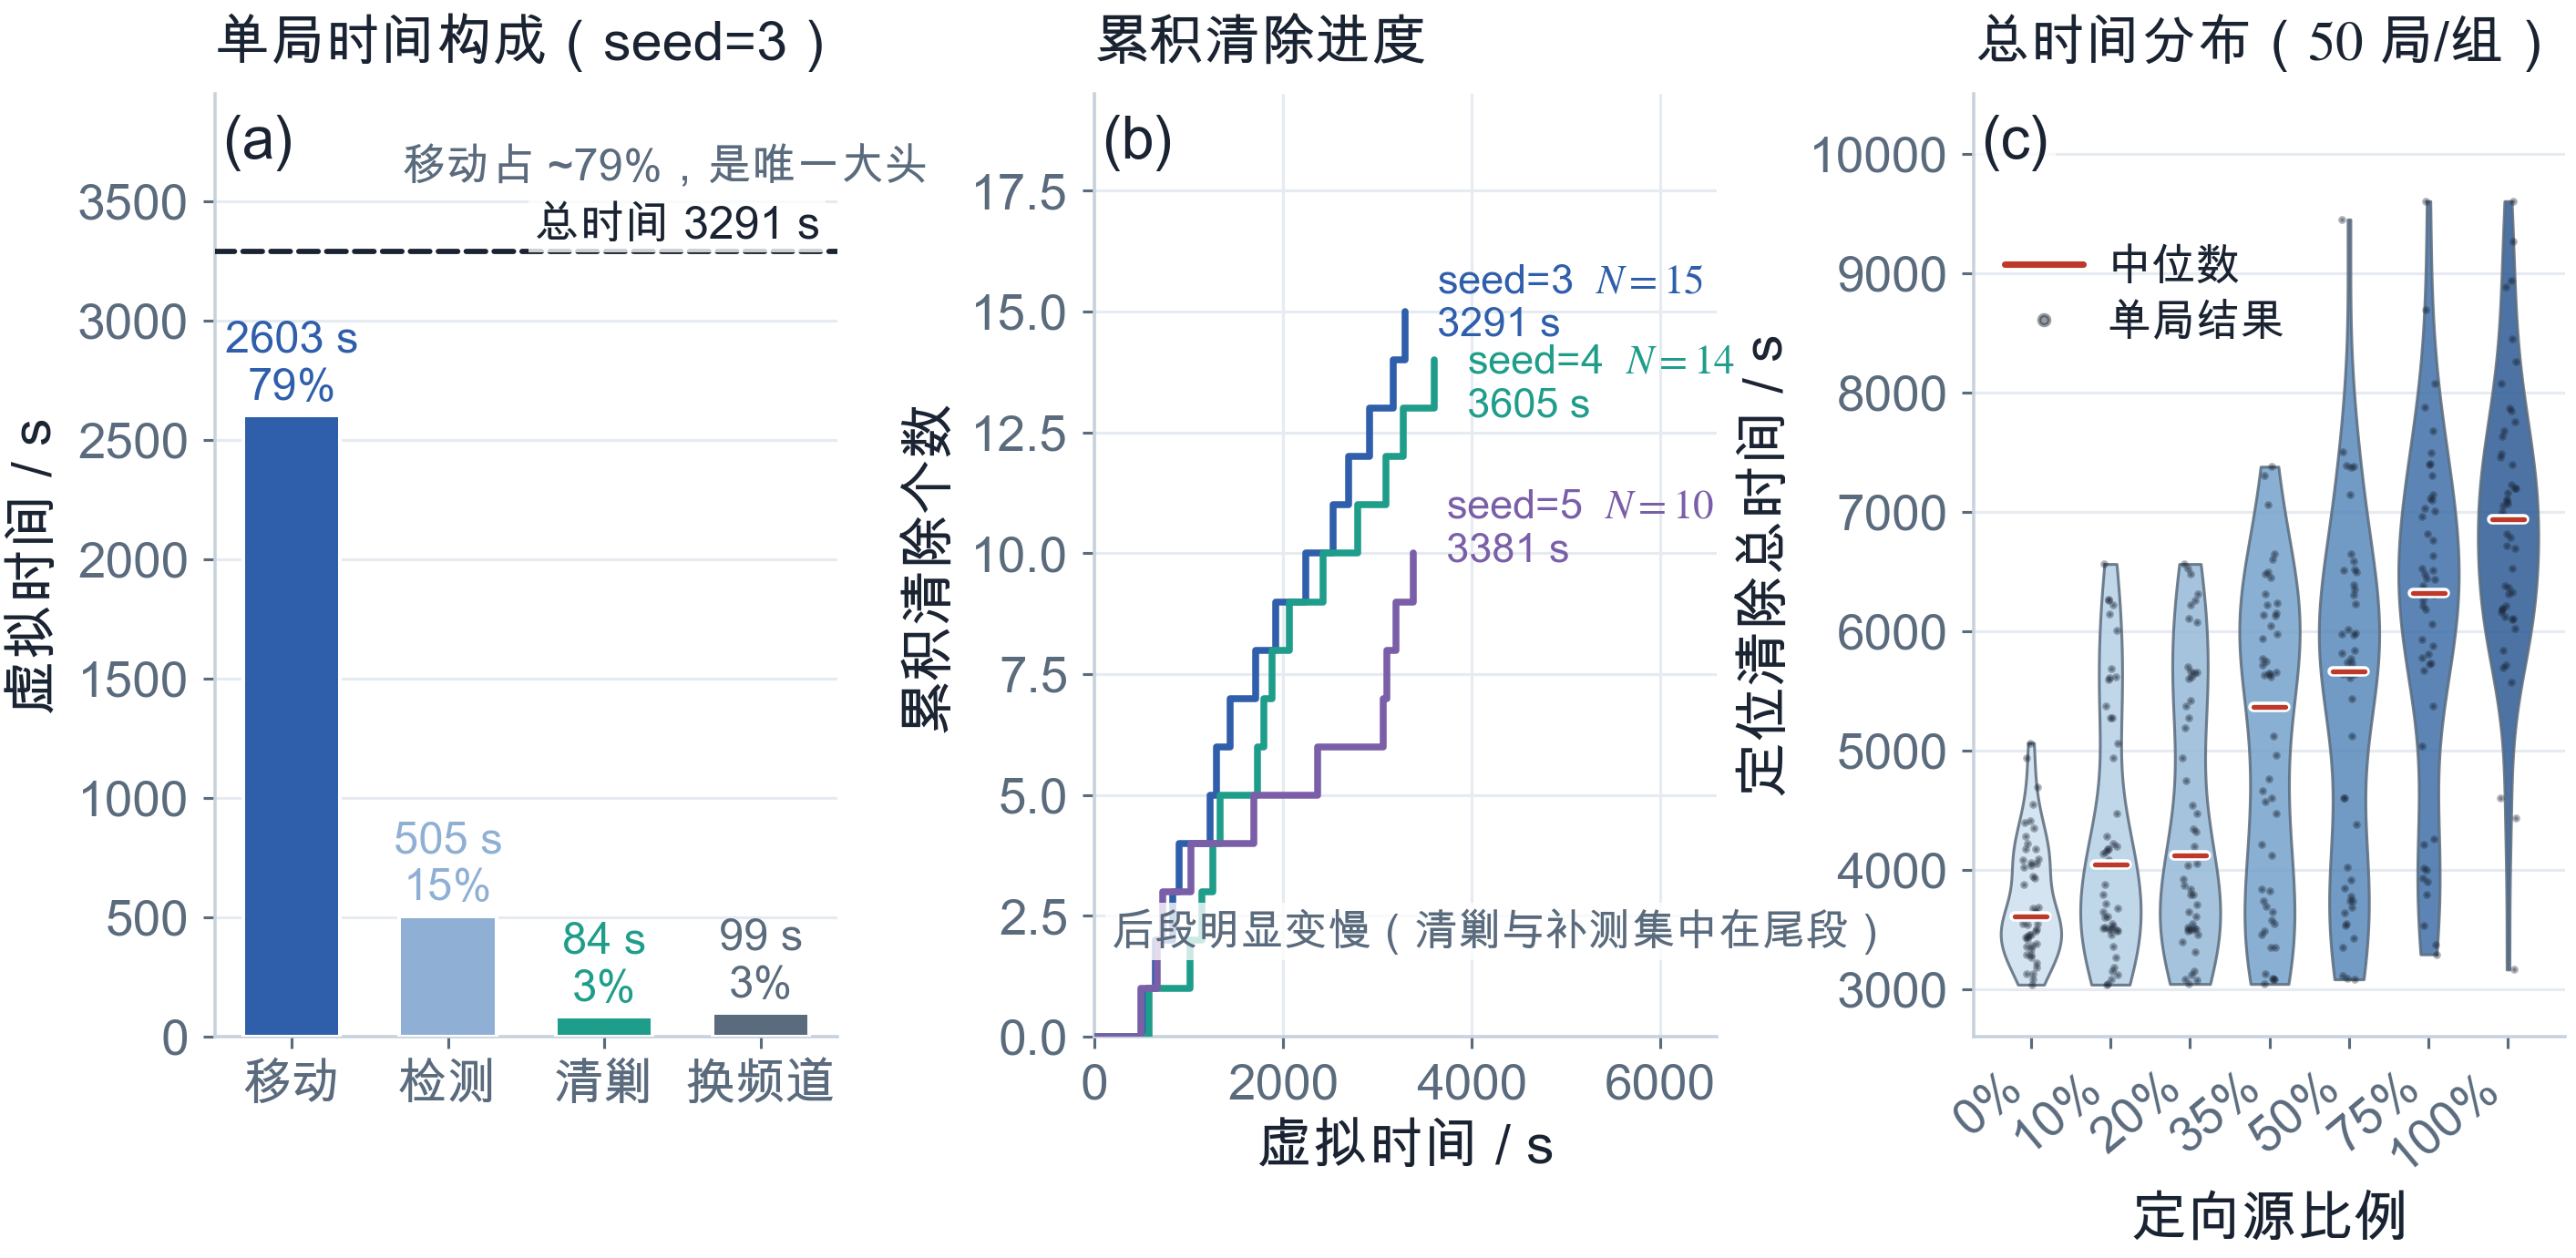
\includegraphics[width=\textwidth]{B_fig5_q3_time.png}
\caption{问题三：(a) 单局时间构成，移动占主导；(b) 累积清除进度；(c) 衔接问题四——总时间分布随定向源比例的变化（各 $50$ 局，$0\%$ 即纯全向场景）}
\label{fig:q3time}
\end{figure}

\subsection{演练测试结果}

在自建模拟器上做 $50$ 局蒙特卡洛演练（源个数 $N\sim U\{10,\dots,16\}$、位置圆盘内均匀、$r_k\sim U[1000,1500]$、频道从 $1\!\sim\!20$ 中无重复抽取），误差场用三种独立模型各测一遍（平滑随机场、独立同分布、分块常值场）：

\begin{table}[H]
\centering
\caption{问题三 演练测试结果（全向干扰源，每组 $50$ 局）}
\label{tab:q3res}
\footnotesize
\setlength{\tabcolsep}{4pt}
\begin{tabular}{@{}lccccccc@{}}
\toprule
误差场模型 & 清除比例 & 全清 & 总时间均值/s & 中位/s & 最短/s & 最长/s & 平均每源/s \\
\midrule
平滑场（$L=1500$ m） & $\bm{100.00\%}$ & $\mathbf{50/50}$ & $3754$ & $3610$ & $3037$ & $5062$ & $293$ \\
平滑场（$L=600$ m）  & $100.00\%$ & $50/50$ & $3722$ & $3613$ & $2976$ & $4938$ & $291$ \\
独立同分布           & $100.00\%$ & $50/50$ & $3744$ & $3634$ & $3001$ & $4962$ & $292$ \\
分块常值场（$200$ m） & $100.00\%$ & $50/50$ & $3727$ & $3614$ & $3015$ & $4957$ & $291$ \\
\bottomrule
\end{tabular}
\end{table}

\noindent\textbf{结果解读}：
\begin{enumerate}
  \item \textbf{$50$ 局全部 $100\%$ 清除}，总时间均值 $3754$ s、中位 $3610$ s、四分位区间 $[3390,4074]$ s，平均每源 $293$ s；
  \item 与 oracle 有效下界 $2307$ s（起点$\,+\,$源$\,+\,$覆盖环）相比，本文策略 $3754$ s 约为其 $\bm{1.63}$ 倍——考虑到策略必须在\emph{未知}源位置的前提下先做搜索、还要付出主动定位的额外移动，这一比值已相当接近可行极限；
  \item \textbf{对误差场模型完全鲁棒}：四种模型下清除率均为 $100\%$、总时间差异 $<1\%$。这并非巧合，而是集值估计的必然结果——策略只使用了 $\pm1^\circ$ 这个\textbf{硬界}，从不假设误差的分布或相关结构（\textbf{这正呼应洞察 1}：把误差当白噪声反而会引入不必要的模型风险）；
  \item 时间构成中\textbf{移动占 $79\%$}（$3754$ s 中约 $2970$ s），检测约 $15\%$、换频道约 $3\%$。故进一步优化的唯一有效方向是压缩路程：本文的滚动重规划把移动由两趟式的 $15\,567$ m 降到 $14\,765$ m，距有效下界 $11\,536$ m 尚有约 $28\%$ 的余量（余量主要来自主动定位与清剿时的局部往返，见第~\ref{sec:q4} 节）。
\end{enumerate}

\subsection{提交与工程实现要点}

\begin{itemize}
  \item \textbf{真实运行时间约束}：题面要求 \texttt{/enter} 后程序运行不超过 $1200$ s、测试窗口 $25$ min。本文策略的单局墙体运行时间远小于 $1$ s（本地仿真），对官方模拟器只需把网络往返控制在可接受范围，并\textbf{限制总请求数}（单局约 $110$ 次 \texttt{/measure} $+$ $16$ 次 \texttt{/clear}）；
  \item \textbf{日志体积}：题面限制加密日志 $\le2$ MB，故客户端只记录必要字段，且对同一 \texttt{request\_id} 的重试\textbf{复用原 payload}（既满足幂等语义，也避免日志膨胀）；
  \item \textbf{坐标范围}：机器狗可以移出目标区域（用于追索区域边缘的源），但坐标分量绝对值不得超过 $2\times10^6$，本文策略自动对候选点做合法域裁剪。
\end{itemize}

\section{问题四：混入定向干扰源后的策略增量}
\label{sec:q4}

\subsection{信息结构发生了什么变化}

全向源与定向源的差别，本质上是 \texttt{no\_signal} 语义的变化：

\begin{equation}
\text{全向源：}\ \texttt{no\_signal}\iff |P_0G|>r_k\ \ge 1000
\quad\Longrightarrow\quad
\text{源在 }\overline{B(P_0,1000)}\text{ 之外（凹约束）};
\end{equation}
\begin{equation}
\text{定向源：}\ \texttt{no\_signal}\iff \underbrace{|P_0G|>r_k}_{\text{太远}}\ \ \text{或}\ \ \underbrace{(G-P_0)^{\!\top}\hat\varphi<0}_{\text{落在阴影半平面}}.
\end{equation}

于是出现两个新现象：

\begin{itemize}
  \item \textbf{区域不再是凸集}：$|P_0G|>1000$ 是圆盘的外部，非凸；与楔形相交后可行域可能分裂成多块，问题一的半平面交算法不再直接适用。本文的处理是\textbf{保守地忽略该约束}（只保留上界可证的部分），保证不漏掉真解——这也与集值估计的"宁可区域大一点、不可丢掉真值"原则一致。
  \item \textbf{"在覆盖内反而收不到"}：这是定向源特有的反常现象，直接威胁问题二的最优解，因为 Q2 的第二点依赖于"第二点能收到信号"。
\end{itemize}

\subsection{核心结论：单圆环对"朝内辐射"的源存在几何盲区}

设源位置 $G=\rho(\cos\alpha,\sin\alpha)$（$\rho=|OG|$）、辐射主方向 $\hat\varphi$（与径向夹角 $\delta$）、环上观测点 $Q=a(\cos\beta,\sin\beta)$。一次检测能收到信号的充要条件是
\begin{equation}
\mathrm{cov}(Q):=\ (G-Q)^{\!\top}\hat\varphi\ \ge\ 0
\quad\Longleftrightarrow\quad
\mathrm{cov}(\beta)=\rho\cos\delta-a\cos(\beta-\delta-\alpha)\ \ge\ 0 .
\label{eq:cov}
\end{equation}

取最不利情形 $\delta=180^\circ$（\textbf{源朝圆心辐射}），此时
\begin{equation}
\boxed{\ \mathrm{cov}(\beta)=-\rho+a\cos(\beta-\alpha)\ \le\ -\rho+a\ <\ 0
\qquad\text{只要}\ \rho>a\ }
\label{eq:blind}
\end{equation}

\textbf{即：当源的半径大于观测环半径、且主方向朝向圆心时，环上任意位置的覆盖判据恒为负——单圆环在几何上永远看不到该源。}

\begin{figure}[H]
\centering
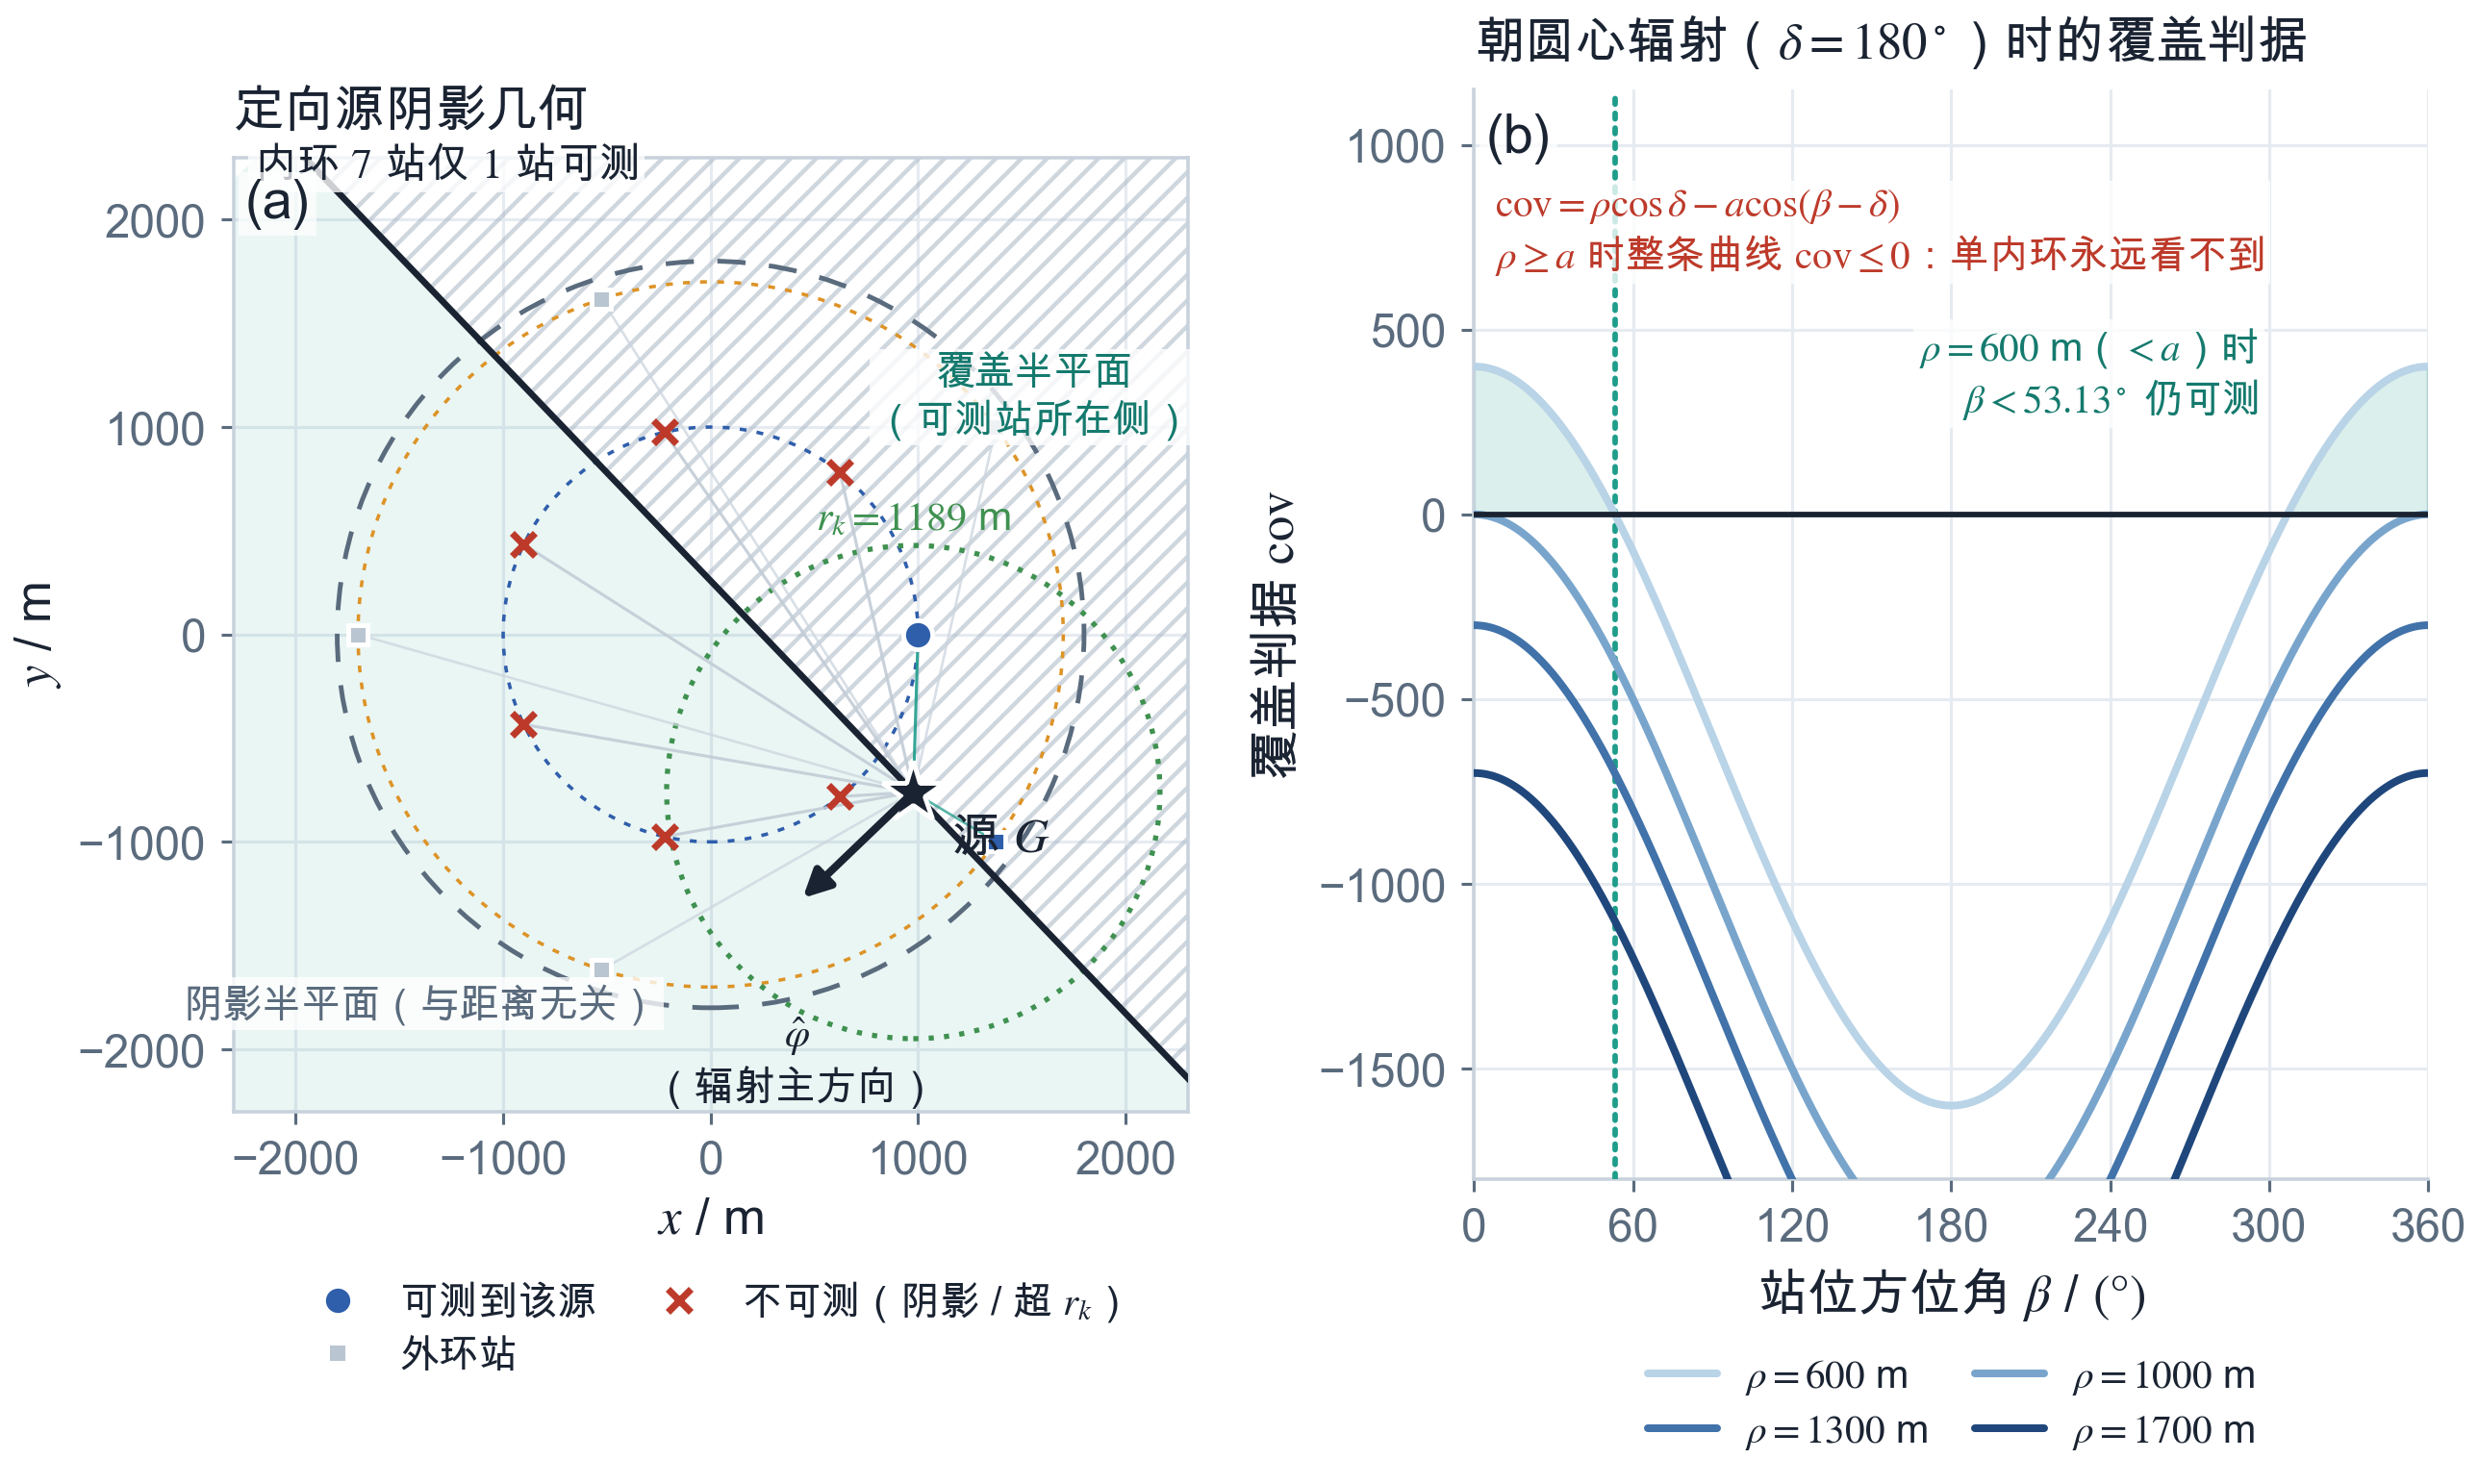
\includegraphics[width=\textwidth]{B_fig6_q4_shadow.png}
\caption{问题四：(a) 一例定向源的阴影几何（$G=(977,-760)$、$r_k=1189$ m、$\hat\varphi=223.8^\circ$），$7$ 个内环站仅 $1$ 个可见；(b) 式~\eqref{eq:blind} 的图解：$\delta=180^\circ$ 且 $\rho\ge a$ 时 $\mathrm{cov}\le0$ 恒成立}
\label{fig:q4shadow}
\end{figure}

图~\ref{fig:q4shadow}(a) 给出实测中的真实例子：源在 $(977,-760)$（$\rho=1238$ m）、$r_k=1189$ m、$\hat\varphi=223.8^\circ$。逐个检查 $7$ 个内环站：站 $0$ $(1000,0)$ 距源 $760$ m 且 $\mathrm{cov}=+543$，\textbf{唯一可测}；站 $6$ $(623,-782)$ 距源仅 $354$ m 却因 $\mathrm{cov}=-270$ 落在阴影中；其余各站或超出 $r_k$、或同时满足两个不利条件。该频道最终\textbf{只有 $1$ 个方位}，直径停在 $\approx1300$ m，永远不会进入清剿队列。

\noindent\textbf{量化影响}：单环策略在定向比例 $100\%$ 时平均只能清除 $7.2$ 个源（真值 $12.96$ 个），清除率仅 $55.0\%$；$35\%$ 时也只有 $81.3\%$。逐局按源类型分解（每组 $50$ 局，\texttt{baseline\_eval.py} 可复现）显示：\textbf{漏掉的源 $100\%$ 都是定向源，全向源的漏检率恒为 $0\%$}，而定向源的漏检率高达 $44.6\%$（$100\%$ 组）、$51.5\%$（$35\%$ 组）。这说明漏检几乎全部是"从未被任何观测点测到"而非"测到了清不掉"——因为清剿环节使用光学/激光定位，与辐射方向无关，\textbf{问题四的难点全部在"测得到"而非"清得掉"}。

\subsection{零成本判据：如何提前知道"这场有定向源"}

外环补扫要额外付出约 $1300$ s 的路程。是否可以只在\emph{确实存在}定向源时才付这笔钱？可以，而且证据是\textbf{免费}的：

\begin{quote}
\textbf{命题 2（定向源判据）} 设某频道已有可行域 $\Reg$（质心 $C$）与至少一个有效方位。记 $\Reg$ 关于质心的\textbf{外接半径}
\begin{equation}
\mathrm{rad}(\Reg):=\max_{v\in\operatorname{vert}(\Reg)}\|v-C\| ,
\label{eq:rad}
\end{equation}
若在点 $Q$ 处该频道返回 \texttt{no\_signal} 且
\begin{equation}
\|Q-C\|+\mathrm{rad}(\Reg)\ <\ r_{\min}=1000\ \text{m},
\label{eq:dircrit}
\end{equation}
则该源\textbf{必为定向源}。
\end{quote}

\noindent\textbf{证明} 反设该源为全向源。$\Reg$ 是凸多边形，而凸集内到定点 $C$ 的最远点必在顶点处取得，故对任意 $G\in\Reg$ 有 $\|C-G\|\le\mathrm{rad}(\Reg)$。于是
$\|Q-G\|\le\|Q-C\|+\|C-G\|\le\|Q-C\|+\mathrm{rad}(\Reg)<1000\le r_k$，
源必落在有效接收半径之内；又因全向源无方向性，$Q$ 处必在覆盖角度内，故必返回 \texttt{direction} 或 \texttt{near}，与 \texttt{no\_signal} 矛盾。$\square$

命题 2 的含义非常实用：\textbf{全向源绝不会在 $1000$ m 内静默，所以在 $1000$ m 内静默的必然是定向源}。这里必须用式~\eqref{eq:rad} 的\emph{精确外接半径}而不是直径的一半：$D/2$ 只是"以质心为中心"的半径的下界，对一般凸多边形 $\mathrm{rad}(\Reg)$ 可以显著超过 $D/2$（例如钝角三角形时 $\mathrm{rad}\to\tfrac23D$），用 $D/2$ 会低估包络、造成\textbf{误触发}。由于 $\Reg$ 是凸多边形，$\mathrm{rad}(\Reg)$ 只须在凸包顶点上取最大值，代价 $O(n)$，与用 $D/2$ 一样廉价，故本文直接取严格值。

实测\textbf{误触发率 $0\%$}：$50$ 局纯全向演练中，判据一次也未触发（表~\ref{tab:q4res} 第 $1$ 行"外环启动率 $0\%$"），因此全向场景的路程与纯单环策略\textbf{完全相同}。这正是我们需要的"按需付费"性质。

\subsection{自适应双环策略}

\begin{quote}
\textbf{算法 4（自适应双环）}
\begin{enumerate}
  \item \textbf{阶段一}：按算法 3 只使用内环 $7$ 站 @$a=1000$ m（表~\ref{tab:cover} 给出的保证覆盖配置），完成扫描 $+$ 滚动清剿；过程中\textbf{实时运行命题 2 的判据}，一旦成立即置位标志 $\mathrm{flag}_{\rm dir}$。
  \item \textbf{阶段二（条件启动）}：仅当 $\mathrm{flag}_{\rm dir}=\text{true}$ 且仍有频道从未获得方位（$\mathrm{n}_{\rm dir}=0$）且已识别数 $<16$ 时，才追加\textbf{外环 $5$ 站 @$a'=1700$ m}（与内环错开 $\pi/5$ 相位），并在其上只对\textbf{未识别频道}做检测。
  \item 外环半径取 $1700$ m 的理由：由式~\eqref{eq:blind}，观测点须满足 $a'>\rho$ 才能进入朝内源的覆盖半平面；由 $\rho\le1800$ m 与 $a'-\rho\le r_{\min}$ 得需 $a'\ge\rho$，取 $a'=1700$ m 可覆盖 $\rho\in[700,1700]$ m 的朝内源（$\rho<700$ m 的朝内源已由内环覆盖；$\rho\in(1700,1800]$ 属于极边缘的少量情形）。
  \item 清剿与主动定位仍按算法 3 执行，其中主动定位点改用式~\eqref{eq:loc} 的\textbf{中等深度双向探测}，并以"正反两侧"作为首选的两个候选（因 $\hat\varphi$ 先验均匀，阴影落在哪一侧等概率，单向尝试等价于 $50\%$ 失效率）。
\end{enumerate}
\end{quote}

\subsection{演练测试结果}

\begin{table}[H]
\centering
\caption{问题四 演练测试结果（每组 $50$ 局，平滑误差场）。基线由 \texttt{baseline\_eval.py} 单因子复现（仅关外环、退回单向补测，种子与本文组完全一致）；"外环启动率"即命题 2 判据触发（\texttt{has\_dir} 置位），也就是外环补扫的闸门打开率}
\label{tab:q4res}
\small
\setlength{\tabcolsep}{4.2pt}
\begin{tabular}{cccccc}
\toprule
定向源比例 & \multicolumn{3}{c}{本文自适应双环策略} & \multicolumn{2}{c}{基线（单环 $+$ 单向补测）} \\
\cmidrule(lr){2-4}\cmidrule(lr){5-6}
 & 清除比例 & 总时间均值 / s & 外环启动率 & 清除比例 & 总时间均值 / s \\
\midrule
$0\%$   & $\bm{100.00\%}$ & $3754$ & $0\%$  & $100.00\%$ & $3661$ \\
$10\%$  & $98.13\%$  & $4291$ & $24\%$ & $95.14\%$  & $3694$ \\
$20\%$  & $96.47\%$  & $4513$ & $32\%$ & $90.97\%$  & $3727$ \\
$35\%$  & $94.25\%$  & $5027$ & $50\%$ & $81.27\%$  & $3772$ \\
$50\%$  & $93.07\%$  & $5371$ & $60\%$ & $76.20\%$  & $3880$ \\
$75\%$  & $91.67\%$  & $6114$ & $78\%$ & $65.38\%$  & $3893$ \\
$100\%$ & $90.86\%$  & $6871$ & $92\%$ & $55.04\%$  & $3932$ \\
\bottomrule
\end{tabular}
\end{table}

\begin{figure}[H]
\centering
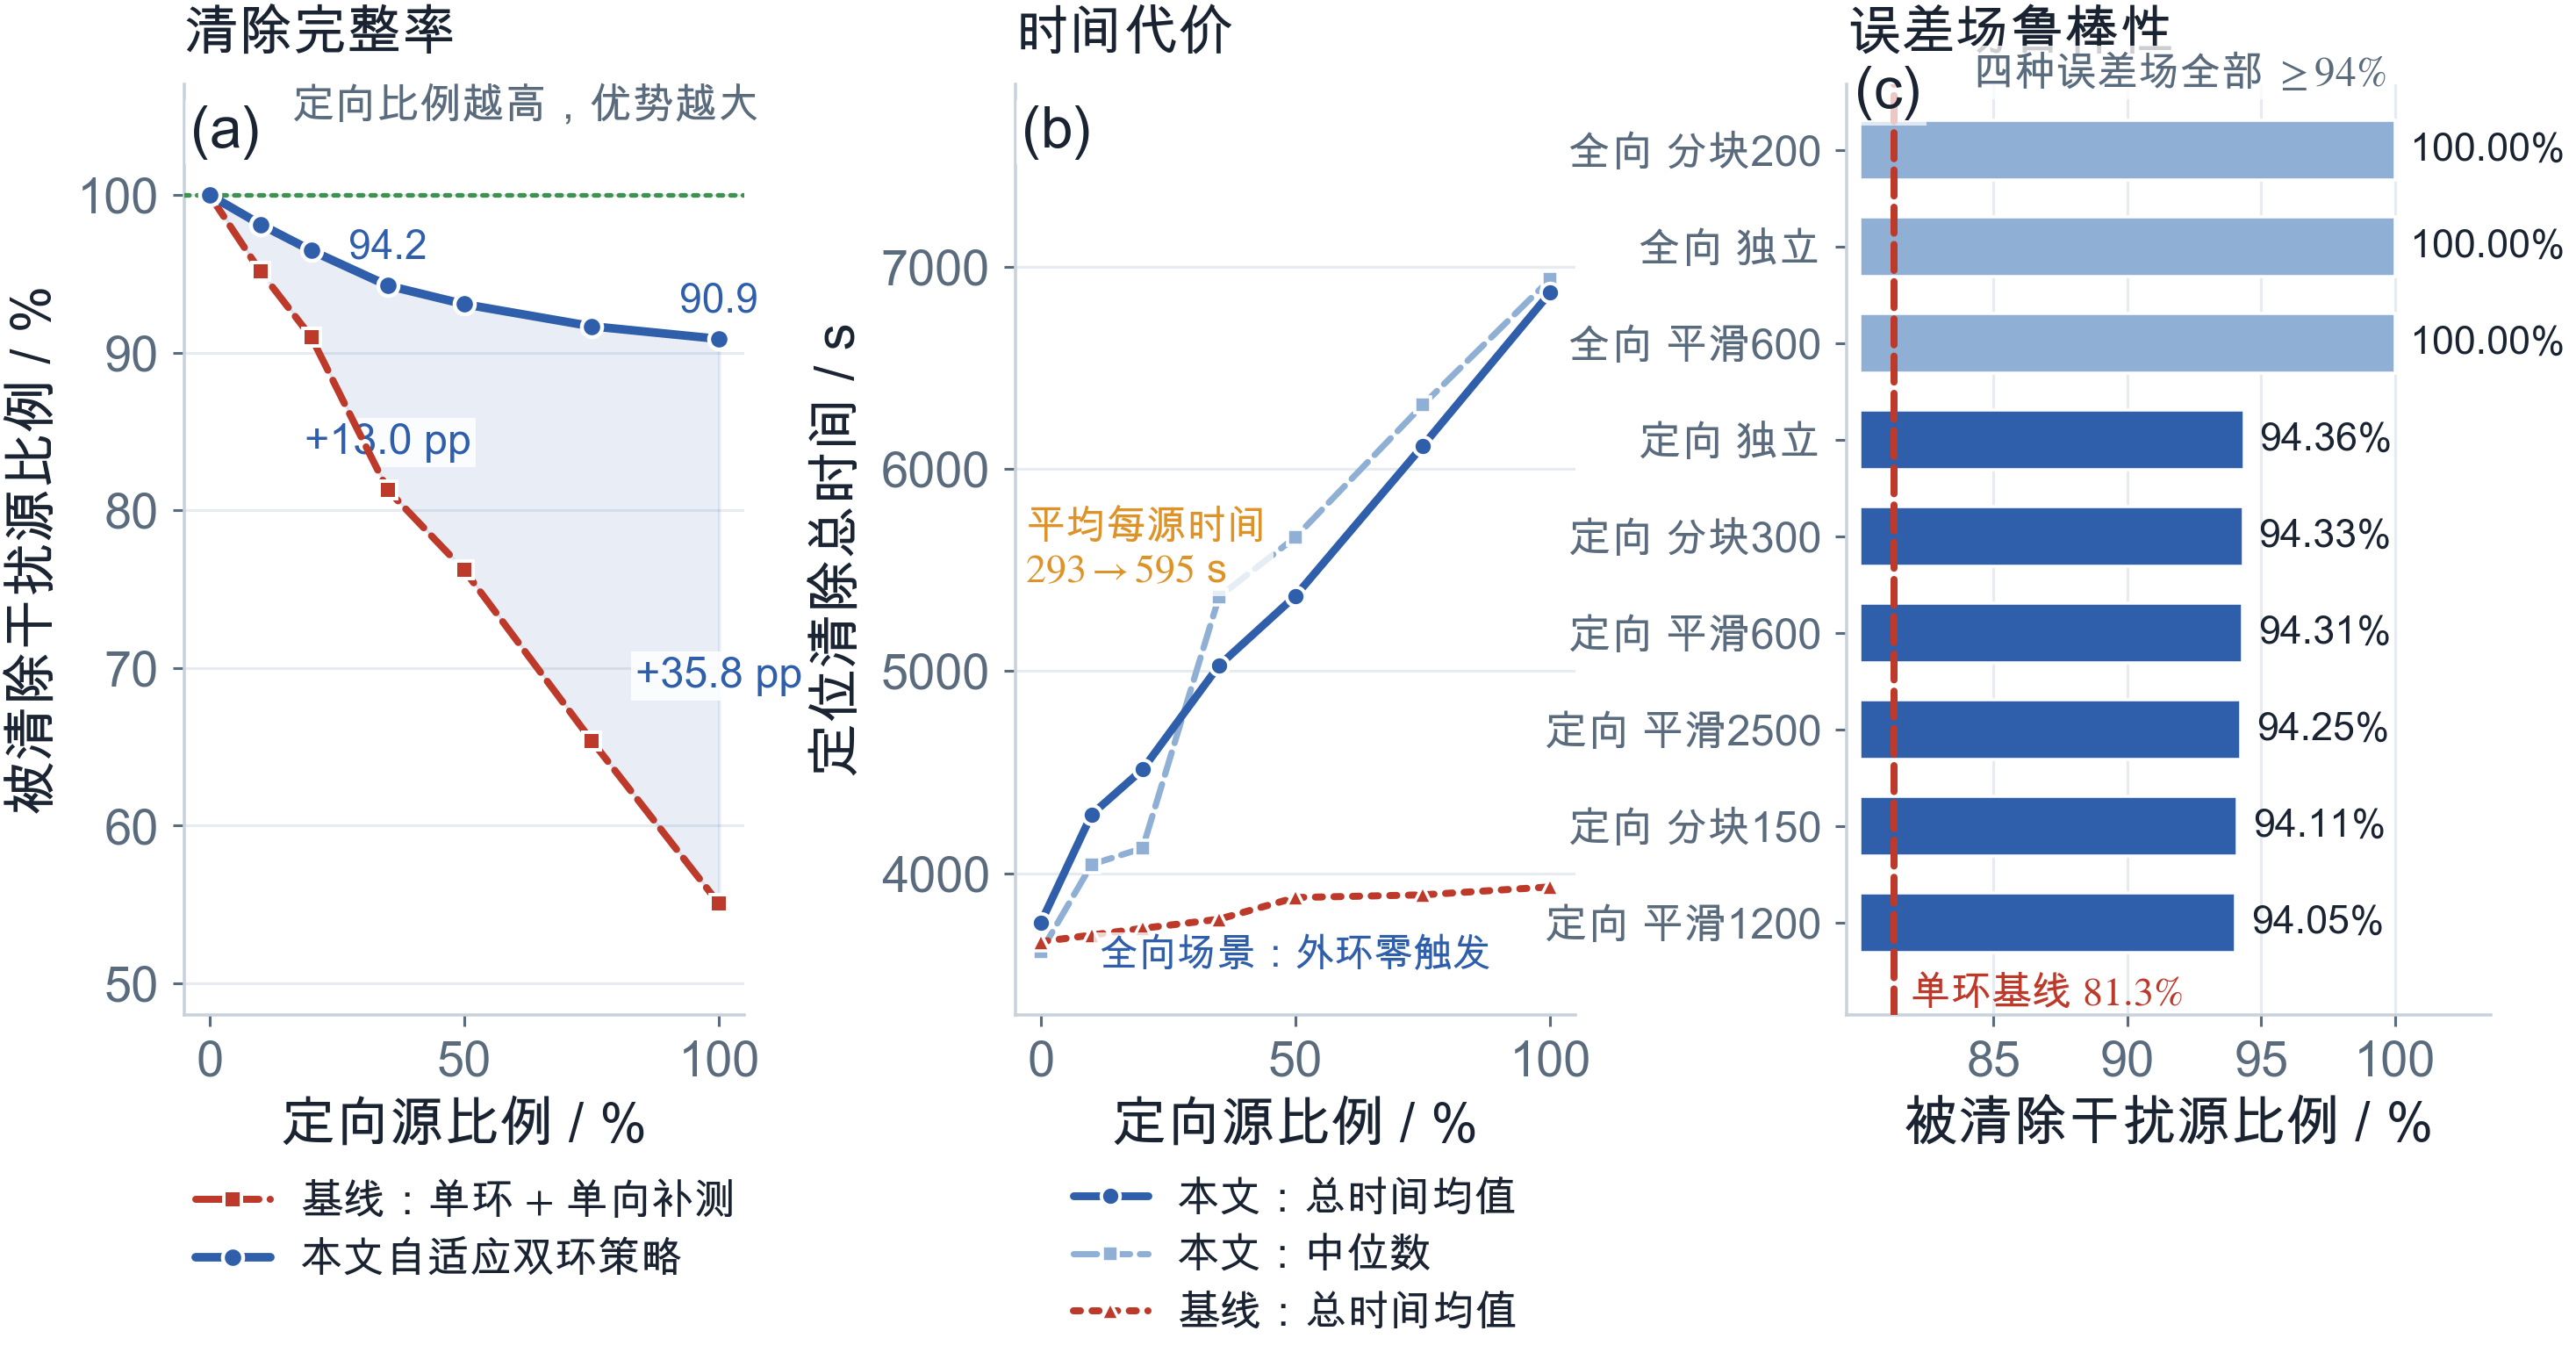
\includegraphics[width=\textwidth]{B_fig7_perf.png}
\caption{性能总结：(a) 清除完整率随定向源比例的变化（与单环基线逐局对比）；(b) 时间代价；(c) 误差场模型鲁棒性}
\label{fig:perf}
\end{figure}

\noindent\textbf{结果解读}：
\begin{enumerate}
  \item \textbf{全向场景零开销}：定向比例 $0\%$ 时判据（式~\eqref{eq:dircrit}）从不触发（$50$ 局触发 $0$ 次），把 \texttt{use\_outer} 打开与关闭得到的 $50$ 局结果\textbf{逐局完全相同}（时间 $3754$ s、移动 $15\,082$ m、检测 $111.4$ 次），与问题三完全一致——\textbf{策略的鲁棒性是"条件自适应"换来的，而不是靠牺牲问题三的性能}。
  \item \textbf{定向场景显著增益}：定向比例 $35\%$ 时清除率由基线的 $\bm{81.3\%}$ 提升到 $\bm{94.25\%}$（$+13.0$ 个百分点），$100\%$ 时由 $\bm{55.0\%}$ 提升到 $\bm{90.86\%}$（$+35.8$ 个百分点）。按源类型逐局分解可知增益的全部来源：\textbf{全向源漏检率两者恒为 $0\%$}，而\textbf{定向源的漏检率由基线的 $51.5\%$（$35\%$ 组）/ $44.6\%$（$100\%$ 组）降到 $16.5\%$/$9.3\%$}——即"把原来漏检掉的那部分定向源重新纳入"。
  \item \textbf{代价可控且"按源计价"不变}：外环仅在需要时启用（$10\%$、$20\%$、$35\%$、$50\%$、$75\%$、$100\%$ 时启动率分别 $24\%$、$32\%$、$50\%$、$60\%$、$78\%$、$92\%$），时间为 $4291\!\sim\!6871$ s，仍远小于 $20$ min 的真实运行约束。值得注意的是$100\%$ 定向组里本文策略平均每源 $595.2$ s，基线为 $592.1$ s，\textbf{几乎相同}——多花的总时间全部换成了多清掉的源，而不是被浪费掉。
  \item \textbf{误差场鲁棒性}：定向 $35\%$ 组在六种误差场配置（平滑场相关长度 $2500$、$1200$、$600$ m，独立同分布，分块常值场 $300$、$150$ m）下清除率为 $94.05\%\!\sim\!94.36\%$、总时间 $5027\!\sim\!5183$ s，\textbf{波动均小于 $3\%$}（图~\ref{fig:perf}c），再次印证集值估计对误差结构的免疫性。
\end{enumerate}

\noindent\textbf{为什么清除率没有到 $100\%$？} 剩余漏检源于式~\eqref{eq:blind} 的两个边界情形：（i）$\rho\in(1700,1800]$ m 且朝内辐射的极边缘源（外环半径 $1700$ m 不足以越过它）；（ii）$r_k$ 恰取下界且几何退化（多个站同时落在阴影内）。这两类都属于"路程预算内不追求绝对保证"的取舍：本文的"内环 $+$ 条件外环"是在"漏检率 $\to0$"与"路程 $\to$ 下界"之间的工程折中，在 $35\%$ 这一题面提示的典型比例下达到 $94.25\%$，且\textbf{全向场景下仍严格 $100\%$}。若场景要求对\emph{任意}（位置, 方向）组合都严格保证"必可测"，则不必依赖任何经验性的加密规则，而存在一个\textbf{可证明的有限站布局}（下一小节的命题 3）；它的路程约为默认方案的一倍，故本文把它作为\emph{按需启用的兜底}，而不是默认方案。

\subsection{\texorpdfstring{严格 $100\%$ 保证}{严格 100\% 保证}：胞元顶点覆盖引理与兜底布局}
\label{sec:complete}

上面"按需付费"的代价是：在极边缘情形下仍有约 $5\%$ 的定向源漏检。若场景要求对\textbf{任意}（位置, 方向）组合都给出 $100\%$ 的"必可测"保证，下面的引理给出了一个干净的构造。

\begin{quote}
\textbf{命题 3（胞元顶点覆盖引理）} 设真值 $G$ 落在胞元 $\conv(V)$ 内，$V=\{v_1,\dots,v_m\}$ 为胞元顶点、同时也被选作观测站；若胞元的\textbf{顶点包络}
\begin{equation}
\max_{i}\|v_i-G\|\ \le\ r_{\min}=1000\ \text{m},
\label{eq:cellcover}
\end{equation}
则对任意辐射主方向 $\hat\varphi$，总存在某个 $v_i$ 使
\begin{equation}
(v_i-G)^{\!\top}\hat\varphi\ \ge\ 0
\quad\text{且}\quad
\|v_i-G\|\ \le\ r_{\min}\ \le\ r_k ,
\label{eq:cellcover2}
\end{equation}
即在 $v_i$ 处一次 \texttt{/measure} \textbf{必能测得该定向源}。
\end{quote}

\noindent\textbf{证明} 因 $G\in\conv(V)$，存在凸组合 $\lambda_i\ge0$、$\sum_i\lambda_i=1$ 使 $G=\sum_i\lambda_i v_i$，故 $\sum_i\lambda_i(v_i-G)=\bm0$。两边点乘 $\hat\varphi$ 得
\[
\sum_i\lambda_i\,(v_i-G)^{\!\top}\hat\varphi=0 .
\]
这是若干\textbf{非负权重}的加权和等于 $0$，故至少有一项非负，即存在 $i$ 满足 $(v_i-G)^{\!\top}\hat\varphi\ge0$；又由式~\eqref{eq:cellcover} 有 $\|v_i-G\|\le r_{\min}\le r_k$。于是该源在 $v_i$ 处同时满足"落在覆盖半平面内"与"在有效接收半径内"两个条件，必返回 \texttt{direction}。$\square$

命题 3 的几何直觉一句话：\textbf{源朝哪个方向辐射，都躲不开它所在胞元的某个顶点}——因为 $G$ 是胞元顶点的凸组合，"各方向加权平均为零"迫使至少一个顶点落在辐射半平面这一侧。它把布局问题彻底化归为\textbf{"让胞元足够小"}：只要胞元内任意点到其顶点的最远距离不超过 $r_{\min}$，就\textbf{不依赖任何概率假设}地保证 $100\%$ 可测。

$\kappa$ 是胞元形状决定的紧常数。本文对每个胞元在 $200^2$ 个源位置采样 $\times$ $1440$ 个方向穷举复算（\texttt{q4\_complete.py}），结果见表~\ref{tab:cell}。

\begin{table}[H]
\centering
\caption{胞元形状与顶点包络紧常数 $\kappa=\sup_{G,\hat\varphi}\min_{i\in T}\|v_i-G\|/h$（$T$ 为落在辐射半平面内的顶点集），数值复算与解析值一致}
\label{tab:cell}
\small
\setlength{\tabcolsep}{5pt}
\begin{tabular}{lccc}
\toprule
胞元形状 & 数值 $\kappa$ & 解析 $\kappa$ & 边长上界 $h_{\max}=r_{\min}/\kappa$ \\
\midrule
正三角形（边长 $h$） & $0.9961$ & $1.0000$ & $1004$ m \\
正方形（边长 $h$）   & $1.1124$ & $\sqrt{5}/2=1.1180$ & $894$ m \\
\bottomrule
\end{tabular}
\end{table}

正方形胞元的最坏情形是：源贴着某侧边的中点、主方向指向胞元内部，此时该侧边的两个顶点都落进阴影半平面，只能用对侧两个顶点，距离为 $\sqrt{h^2+(h/2)^2}=\tfrac{\sqrt5}{2}h$；正三角胞元的最坏值恰为 $h$（源趋近某一顶点、主方向沿对边方向），故\textbf{三角格在同一保证标准下允许更粗的间距、更少的站}。

据此取 $h=950$ m 的\textbf{三角格}（$\Arena$ 内加界外顶点共 $31$ 站，站间距 $950$ m $\cdot$ $\kappa=946$ m $<1000$ m，留 $54$ m 余量），按命题 3 即可对任意（位置, 方向）组合保证可测。表~\ref{tab:complete} 给出它与方格布局的代价对比（巡回长度为自圆心出发的最近邻 $+$ 2-opt）。

\begin{table}[H]
\centering
\caption{严格保证布局的站数与巡回代价（\texttt{q4\_complete.py} 复算；每种布局各做 $2\times10^5$ 次随机（位置, 方向）抽样，失败率均为 $0$）}
\label{tab:complete}
\small
\setlength{\tabcolsep}{4.5pt}
\resizebox{\linewidth}{!}{%
\begin{tabular}{lccccc}
\toprule
布局 & 站数 & 失败率 & 最近可测站距/m & 巡回/m & 时间/s \\
\midrule
\textbf{三角格 $h=950$ m（兜底）} & $\bm{31}$ & $0\%$ & $948.9$ & $\bm{29\,195}$ & $5839$ \\
三角格 $h=1000$ m & $31$ & $0\%$ & $999.0$ & $31\,464$ & $6293$ \\
方格 $h=850$ m & $45$ & $0\%$ & $941.0$ & $38\,456$ & $7691$ \\
方格 $h=600$ m & $69$ & $0\%$ & $662.6$ & $41\,794$ & $8359$ \\
\bottomrule
\end{tabular}}
\end{table}

\noindent\textbf{为什么本文默认不启用它？} 三角格兜底布局的巡回为 $29\,195$ m $=5839$ s，\emph{仅路程}就已是主策略全向总时间（$3754$ s）的 $1.56$ 倍；再考虑到保证来源于"某个站必能看到"、事先并不知道是哪个站，必须对每个站点逐频道扫描，检测开销也会明显上升。因此本文的工程结论是：\textbf{默认用"内环 $+$ 条件外环"以 $3754\!\sim\!6871$ s 清掉 $91\%\!\sim\!100\%$ 的源；仅在"判据确已证实存在定向源、常规手段停滞、且已知定向比例上界偏高"时，才切换到三角格兜底布局}，用约一倍的路程换取 $100\%$ 的\emph{可测}保证。这种"保证等级可调"的设计也是集值估计路线的自然延伸——\textbf{漏检率与路程可以显式地对换，而不是靠调参碰运气}。

\section{模型评价与推广}

\subsection{模型优点}

\begin{enumerate}
  \item \textbf{数学结构清晰、结论可证}：全题建立在"集值估计 $+$ 凸几何"之上，问题一的 Thales 判据、Jung 上界、问题四的几何盲区定理（式~\eqref{eq:blind}）都是可证明的严格结论，而非调参经验；
  \item \textbf{误差模型无关的鲁棒性}：策略只用 $\pm1^\circ$ 硬界，对平滑场/独立同分布/分块场全部给出 $100\%$（全向）与 $\approx94.2\%$（定向 $35\%$）的一致结果，避免了"把确定性误差当白噪声"这一常见建模错误；
  \item \textbf{闭环可执行}：算法输出的是可直接下发的 \texttt{/measure}、\texttt{/clear} 坐标序列；策略与模拟器通过 \texttt{transport} 接口解耦，换成 HTTP 传输即可对官方模拟器运行；
  \item \textbf{逼近理论下界}：全向场景总时间 $3754$ s、移动 $15\,082$ m，与"起点$\,+\,$源$\,+\,$覆盖环"的有效下界 $11\,536$ m 相差 $31\%$（时间约为该下界的 $1.63$ 倍）；
  \item \textbf{条件自适应}：问题四的额外代价只在该付的时候付（全向场景判据零误触发）。
\end{enumerate}

\subsection{模型缺点与改进方向}

\begin{enumerate}
  \item \textbf{\texttt{no\_signal} 的凹信息被保守丢弃}：全向场景下"$|P_0G|>1000$"是有效的排除信息，本文为保持凸性而未使用，导致可行域偏大、检测次数偏多。改进方向：用"凸分解 $+$ 分支定界"或"外逼近"处理非凸约束，预计可再省 $10\%\!\sim\!15\%$ 检测次数；
  \item \textbf{定向源默认策略仍未 $100\%$ 保证}：如第~\ref{sec:complete} 节所述，$100\%$ 的可测保证需要"胞元顶点包络 $\le r_{\min}$"的加密布局（三角格 $h=950$ m、$31$ 站，巡回 $29\,195$ m），其路程约为默认方案的一倍，故本文仅把它作为按需启用的兜底；若要常态化启用，可进一步用"变密度格"（在 $\rho\in(1700,1800]$ m 的边缘环带局部加密、内部放粗）把站数再压下去；
  \item \textbf{路径规划为启发式}：滚动最近邻 $+$ $2$-opt 在 $20\!\sim\!25$ 个点的规模下与最优解差距约 $5\%\!\sim\!10\%$；若允许更多在线计算，可用 LKH/Held--Karp 或"插入式增量 TSP"；
  \item \textbf{$r_k$ 的先验利用不足}：多次观测同一源可以反推 $r_k$ 的区间（"测得到"给下界、"测不到"给上界），进而收紧其他频道的推理，本文未展开。
\end{enumerate}

\subsection{推广}

本文的"集值可行域 $\to$ 直径作为不确定度 $\to$ 最优观测点设计 $\to$ 滚动调度"链条可直接迁移到：

\begin{itemize}
  \item \textbf{室内定位/室内机器人}：WiFi/蓝牙指纹定位中"同点重复测量一致、跨点呈统计规律"的误差同样应作集值处理；
  \item \textbf{声呐/雷达搜潜}：探测方位误差为确定性偏差时的交会定位与搜索路径规划；
  \item \textbf{无人机搜寻救援}：有限探测半径 $+$ 遮蔽（对应本文的定向阴影）下的目标搜索；
  \item \textbf{传感器网络布设}：式~\eqref{eq:cover} 的"保证覆盖"不等式给出了给定探测半径与区域半径下最少节点数及其半径区间，可直接用于工程选型。
\end{itemize}

\begin{thebibliography}{9}
\bibitem{jung} Jung H W E. Über die kleinste Kugel, die eine räumliche Figur einschliesst[J]. Journal für die reine und angewandte Mathematik, 1901, 123: 241--257.
\bibitem{welzl} Welzl E. Smallest enclosing disks (balls and ellipsoids)[C]// New Results and New Trends in Computer Science. Springer, 1991: 359--370.
\bibitem{prep} Preparata F P, Shamos M I. Computational Geometry: An Introduction[M]. Springer, 1985.
\bibitem{sh} Sutherland I E, Hodgman G W. Reentrant polygon clipping[J]. Communications of the ACM, 1974, 17(1): 32--42.
\bibitem{croes} Croes G A. A method for solving traveling-salesman problems[J]. Operations Research, 1958, 6(6): 791--812.
\bibitem{bhh} Beardwood J, Halton J H, Hammersley J M. The shortest path through many points[J]. Mathematical Proceedings of the Cambridge Philosophical Society, 1959, 55(4): 299--327.
\bibitem{gal} Gal S. Search games[M]. Academic Press, 1980.
\bibitem{chvatal} Chvátal V, Cook W J. The Traveling Salesman Problem: A Computational Study[M]. Princeton University Press, 2006.
\end{thebibliography}

\newpage
\appendix

\section{支撑材料文件列表}

\begin{table}[H]
\centering
\caption{自建代码与数据文件清单（路径均相对参赛仓库根目录）}
\label{tab:files}
\footnotesize
\setlength{\tabcolsep}{4pt}
\begin{tabular}{@{}cl >{\raggedright\arraybackslash}p{7.4cm}@{}}
\toprule
序号 & 文件 & 说明 \\
\midrule
1 & \texttt{jammer\_sim.py} & 自建等价模拟器：$\mathcal A$、误差场、\texttt{Simulator}、\texttt{LocalTransport}/\texttt{HttpTransport}、\texttt{RobotClient} \\
2 & \texttt{strategy.py} & 策略主体：\texttt{Region}（半平面交）、\texttt{chan} 状态、站点布局、滚动重规划主循环、主动定位、清剿 \\
3 & \texttt{selftest.py} & 计时规则自检（复现附件 1 表 2 的 $105$、$111$、$194$、$199$ s 四个时刻） \\
4 & \texttt{final\_eval.py} & 问题三/四演练测试与鲁棒性批量评估，输出 \texttt{results/*.csv} \\
5 & \texttt{baseline\_eval.py}、\texttt{order\_ablation.py} & 单环基线对照实验、任务顺序/主动定位消融（表~\ref{tab:q4res} 与两趟式对比的产出脚本） \\
6 & \texttt{q3\_bounds.py} & 覆盖环几何与 oracle 下界的独立复算（表~\ref{tab:cover} 与下界表的产出脚本） \\
7 & \texttt{q4\_complete.py} & 问题四严格保证的独立复算：命题 3 的紧常数 $\kappa$、三角格/方格布局的站数、$2\times10^5$ 次（位置, 方向）抽样验证与巡回长度（表~\ref{tab:cell}、\ref{tab:complete}） \\
8 & \texttt{scan.py}、\texttt{run\_mc.py} & 参数扫描与单组蒙特卡洛 \\
9 & \texttt{probe/B\_probe*.py} & 问题一、二的独立几何验证（直径、最小包围圆、Jung 上界、$J$ 曲面） \\
10 & \texttt{figs/make\_figs\_B*.py} & 全部插图生成脚本（可复现） \\
11 & \texttt{results/*.csv}、\texttt{*.npz} & $1100$ 余局演练的逐局明细 \\
12 & \texttt{paper/main.tex}、\texttt{refs} & 论文 \LaTeX{} 源码与参考文献 \\
\bottomrule
\end{tabular}
\end{table}

\section{核心源程序}

\subsection{可行域与直径（问题一核心）}

\begin{verbatim}
class Region:
    """可行域：凸多边形。只用"楔形 + 圆盘"两类凸约束（no_signal 是凹约束，保守忽略）。"""
    def _clip(self, a, b, c):
        poly = self.poly
        if not poly: return
        out, n = [], len(poly)
        for i in range(n):
            P, Q = poly[i], poly[(i + 1) % n]
            fp, fq = a * P[0] + b * P[1] - c, a * Q[0] + b * Q[1] - c
            if fp <= 0: out.append(P)
            if (fp < 0 < fq) or (fq < 0 < fp):
                t = fp / (fp - fq)
                out.append((P[0]+t*(Q[0]-P[0]), P[1]+t*(Q[1]-P[1])))
        self.poly = out

    def add_wedge(self, S, theta_deg, half_deg=EPS_DEG):
        """2° 楔形 -> 两条边界射线的同侧半平面约束。法向符号由"楔内测试点"确定。"""
        t = math.radians(theta_deg); d = math.radians(half_deg)
        p_in = np.array([S[0]+300.0*math.cos(t), S[1]+300.0*math.sin(t)])
        Sn = np.asarray(S, float)
        for tb in (t - d, t + d):
            n = np.array([-math.sin(tb), math.cos(tb)])
            if n @ (p_in - Sn) < 0: n = -n
            self._clip(-n[0], -n[1], -(n @ Sn))

    def add_disk(self, S, R, n=DISK_N):
        """半径 R 的接收圆盘（内接正 n 边形近似）。"""
        for k in range(n):
            mid = 2 * math.pi * (k + 0.5) / n
            nx, ny = math.cos(mid), math.sin(mid)
            self._clip(nx, ny, nx * S[0] + ny * S[1] + R)

    def diameter(self):
        """凸多边形直径：顶点枚举（n 很小），返回 (D, A, B)。"""
        V = self.hull(); best = (-1.0, None, None)
        for i in range(len(V)):
            for j in range(i + 1, len(V)):
                d = math.hypot(V[j][0] - V[i][0], V[j][1] - V[i][1])
                if d > best[0]: best = (d, V[i], V[j])
        return best
\end{verbatim}

\subsection{滚动重规划主循环（问题三核心）}

\begin{verbatim}
def _actions(self, st, pending_st):
    """候选任务集：扫描站 st / 主动定位 loc / 清剿 cl。
    优先级规则（Q2 结论的工程落地）：只要还有未扫的圆环站就先扫站——
    相邻站基线 2a*sin(pi/m) ~ 708 m，与 ~900 m 处的源构成 ~47° 交会角，
    单次观测即把 D 从 1300 m 压到 ~22 m，远优于"在质心附近小偏置补测"。"""
    acts = [(np.asarray(S, float), "st", -1) for S in pending_st]
    have_st = bool(pending_st)
    for ch in range(1, 21):
        c = st[ch]
        if c.cleared or c.n_dir == 0: continue
        if self._ready(c):
            acts.append((c.reg.centroid(), "cl", ch))
        elif c.n_loc < self.P["max_loc"] and (\
                c.n_dir >= self.P["loc_min_dir"] or not have_st):
            acts.append((self._loc_point(c), "loc", ch))
    return acts

def run(self, client):
    """滚动重规划：每步只走 2-opt 巡回的第一站，随后按新信息重排。"""
    st = {ch: Chan.fresh() for ch in range(1, 21)}
    pos = np.array([0.0, 0.0]); client.enter()
    inner = ring_stations(self.P["ring_m"], self.P["ring_a"], self.P["ring_rot"])
    outer = ring_stations(self.P["ring_m2"], self.P["ring_a2"],
                          self.P["ring_rot"] + math.pi / self.P["ring_m2"])
    pending_st = [np.asarray(s, float) for s in tour(inner)]
    while it < self.P["max_iter"]:
        acts = self._actions(st, pending_st)
        if not acts and not pending_st and outer and self.P["use_outer"] \
                and self.has_dir and self.n_det < self.P["n_max"] \
                and any(st[ch].n_dir == 0 for ch in range(1, 21)):
            # 阶段二：仅在"已证实存在定向源"时启动外环补扫（命题 2 的判据）
            pending_st = [np.asarray(s, float)
                          for s in tour(outer, start=pos)]
            outer = None; acts = self._actions(st, pending_st)
        if not acts: break
        pts = [a[0] for a in acts]
        first = np.asarray(tour(pts, start=pos)[0], float)      # 滚动视界，只取首站
        k = min(range(len(acts)),
                key=lambda i: float(np.linalg.norm(pts[i]-first)))
        _, kind, ch = acts[k]
        if kind == "st":
            pos = self._sweep(client, pts[k], st, pos)
            pending_st = [S for S in pending_st
                          if float(np.linalg.norm(np.asarray(S,float)-pts[k])) > 1e-6]
        elif kind == "loc":
            pos = self._locate(client, ch, st[ch], pos)
        else:
            ok, pos = self._clear(client, ch, st[ch], pos)
    client.exit()
\end{verbatim}

\subsection{定向源判据与双环触发（问题四核心）}

\begin{verbatim}
def _update(self, st, x, y, resp):
    res = resp.get("measure_result")
    if res == "direction":
        st.reg.add_wedge((x, y), float(resp["svd_deg"]))
        st.reg.add_disk((x, y), R_RECV_MAX)
        st.obs.append((x, y, resp["svd_deg"]))
        st.n_dir += 1
    elif res == "near":
        st.reg.add_disk((x, y), 5.0, n=24); st.n_dir += 1
    else:
        st.n_nosig += 1
        # 【命题 2】全向源只要 |QG| <= r_k 必有信号，而 r_k >= 1000 m，
        # 故"在距源 < 1000 m 处仍 no_signal"只可能来自定向源的阴影半平面。
        # 严格包络：不能用 D/2（它只是以质心为心的半径的下界，见命题 2 注）。
        # 可行域是凸多边形 -> max|g-C| 必在凸包顶点取得，直接算精确外接半径。
        if st.n_dir > 0:
            H = st.reg.hull()
            if len(H) >= 3:
                C = st.reg.centroid()
                rho_max = max(math.hypot(v[0] - C[0], v[1] - C[1]) for v in H)
                if math.hypot(x - C[0], y - C[1]) + rho_max < R_RECV_MIN:
                    self.has_dir = True      # 置位 -> 允许启动外环补扫
    return res
\end{verbatim}

\subsection{自建模拟器的计时核心（与附件 1 逐秒吻合）}

\begin{verbatim}
if path == "/measure":
    sw = 0.0
    if ch != self.chan:                 # 相邻两次 measure 频道不同 -> 切换耗时 1 s
        sw = T_SWITCH; self.n_switch += 1
    self.t += mv + sw + T_MEASURE       # mv = d/5
    self.chan = ch
else:                                   # /clear
    self.t += mv + T_CLEAR_FAIL         # 未发现：3 s
    ok = (idx is not None and idx not in self.cleared
          and float(np.linalg.norm(self.case.pos[idx] - p)) <= R_CLEAR)
    if ok:
        self.cleared.add(idx)
        self.t += (T_CLEAR_OK - T_CLEAR_FAIL)   # 成功：再 +2 s
    # 注意：/clear 不改变 self.chan，也不产生切换耗时
\end{verbatim}



\end{document}
